\documentclass[11pt,a4paper]{report}
\usepackage[portuges]{babel}
\usepackage[utf8]{inputenc} % define o encoding usado texto fonte (input)--usual "utf8" ou "latin1
\usepackage{graphicx} %permite incluir graficos, tabelas, figuras
\usepackage{subcaption}
\usepackage{listings}
\usepackage{color}
\usepackage{multicol}
\usepackage{indentfirst}
\usepackage{hyperref}
\usepackage{amsmath}
\usepackage{amssymb}
\usepackage{float}
\usepackage{enumitem}
\usepackage{tabularx}
\usepackage{atbegshi}
\parskip=2pt % espaço entre o parágrafo e o texto anterior

\setlength{\oddsidemargin}{-1cm} %espaço entre o texto e a margem
\setlength{\textwidth}{18cm} %Comprimento do texto na pagina
\setlength{\headsep}{-1cm} %espaço entre o texto e o cabeçalho
\setlength{\textheight}{23cm} %altura do texto na pagina


\definecolor{myblue}{rgb}{0.2,0.2,0.8}
\definecolor{mygray}{rgb}{0.5,0.5,0.5}
\definecolor{mymauve}{rgb}{0.58,0,0.82}

\lstdefinestyle{code}{ 
  backgroundcolor=\color{white},   % choose the background color; you must add \usepackage{color} or \usepackage{xcolor}; should come as last argument
  basicstyle=\footnotesize,        % the size of the fonts that are used for the code
  breakatwhitespace=false,         % sets if automatic breaks should only happen at whitespace
  breaklines=true,                 % sets automatic line breaking
  captionpos=b,                    % sets the caption-position to bottom
  commentstyle=\color{white},    % comment style
  deletekeywords={...},            % if you want to delete keywords from the given language
  escapeinside={\%*}{*)},          % if you want to add LaTeX within your code
  extendedchars=true,              % lets you use non-ASCII characters; for 8-bits encodings only, does not work with UTF-8
  firstnumber=1000,                % start line enumeration with line 1
  keepspaces=true,                 % keeps spaces in text, useful for keeping indentation of code (possibly needs columns=flexible)
  keywordstyle=\color{blue},       % keyword style
  language=C++,                 % the language of the code
  morekeywords={*,...},            % if you want to add more keywords to the set
  numberstyle=\tiny\color{mygray}, % the style that is used for the line-numbers
  rulecolor=\color{black},         % if not set, the frame-color may be changed on line-breaks within not-black text (e.g. comments (green here))
  showspaces=false,                % show spaces everywhere adding particular underscores; it overrides 'showstringspaces'
  showstringspaces=false,          % underline spaces within strings only
  showtabs=false,                  % show tabs within strings adding particular underscores
  stepnumber=2,                    % the step between two line-numbers. If it's 1, each line will be numbered
  stringstyle=\color{mymauve},     % string literal style
  tabsize=2,                     % sets default tabsize to 2 spaces
  title=\lstname                   % show the filename of files included with \lstinputlisting; also try caption instead of title
}

\AtBeginDocument{\AtBeginShipoutNext{\AtBeginShipoutDiscard}}

\title{Projeto - ComputationalMind\\ Desafios para Desenvolvimento  Computacional} %Titulo do documento

\author{Inês Pires Presa (A90355)\and Ivo Miguel Gomes Lima (A90214)\and Tiago André Oliveira Leite (A91693)\and Tiago dos Santos Silva Peixoto Carriço (A91695)} %autores do documento

\date{\today} %data

\begin{document}
\pagenumbering{gobble}
\clearpage
\thispagestyle{empty}

  \begin{minipage}{0.9\linewidth}
        \centering
    
\includegraphics[width=0.4\textwidth]{um.jpeg}\par\vspace{1cm}
                \href{https://www.uminho.pt/PT}
    {\scshape\LARGE Universidade do Minho} \par
    \vspace{0.6cm}
                \href{https://lcc.di.uminho.pt}
    {\scshape\Large Licenciatura em Ciências da Computação} \par
    \maketitle
    \begin{center}
      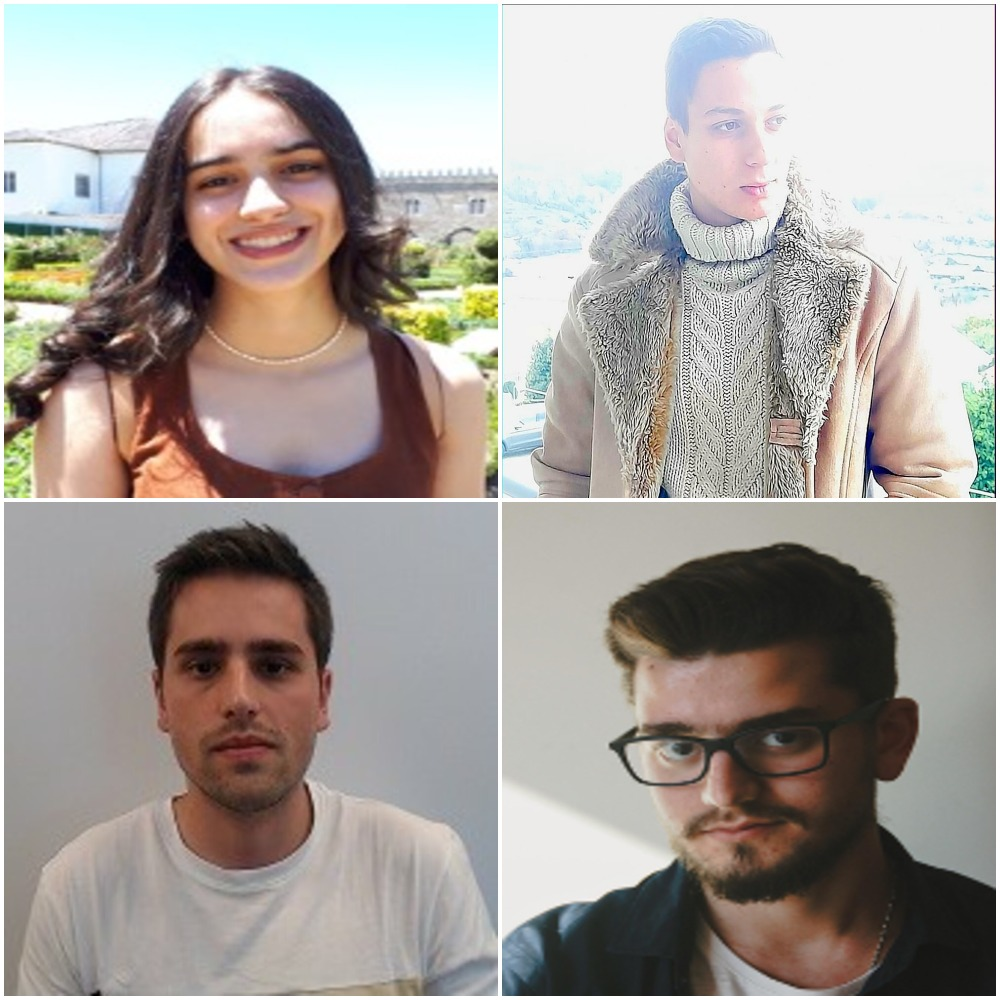
\includegraphics[width=0.7\linewidth]{us.jpg}
\end{center}
  \end{minipage}

\begin{abstract}  % resumo do documento

Este relatório retrata todo o processo de desenvolvimento da plataforma \emph{“ComputationalMind”} e as diferentes decisões tomadas ao longo do mesmo. O objetivo deste projeto é criar um \emph{Website} educacional para uso em escolas e outras instituições de ensino, que possibilite ao público mais jovem aprender por meio de jogos de escolha múltipla, resposta curta e verdadeiro ou falso, o \emph{mindset} a adotar para ser um excelente \emph{problem solver} e, consequentemente, um excelente programador.
O desenvolvimento começou pelo desenho do modelo lógico da base de dados e validação da mesma junto dos proponentes. Para tal foram  utilizadas as ferramentas \emph{draw.io} e \emph{MySQL WorkBench}. A implementação física da base de dados foi realizado através da \emph{framework Django} e o sistema de gestão de bases de dados escolhido foi o \emph{MySQL}.
O \emph{back-office} foi construido em \emph{Django} com recurso à ferramenta \emph{Django rest framework} que possibilita o desenvolvimento de \emph{Web APIs}. O
\emph{front-office} foi feito com \emph{ReactJS} e \emph{tailwindcss} sendo que o seu processo de construção começou com o desenho de \emph{mockups} no \emph{figma.com}.
O fluxo dos dados inseridos pelo utilizador é feita do \emph{front-office} para o \emph{back-office} pela \emph{rest API} através de ficheiros \emph{Json}. Os dados enviado pelo \emph{ReactJS} são recebido pelo \emph{Django}, validados e caso estejam no formato correcto, são inseridos na base de dados. O fluxo de dados da BD para o utilizador é realizada de modo análogo.
A plataforma pode ser acedida por meio de um navegador \emph{web} no computador ou telemóvel.\newline\newline

\textbf{Palavras-Chave:} Pensamento Computacional, \emph{web site}, aprendizagem,  \emph{back-office}, \emph{front-office}, \emph{back-end}, \emph{front-end} \emph{Rest framework}, \emph{Django}, \emph{ReactJS}, \emph{Base de dados}.

\end{abstract}

\tableofcontents % insere Indice

\chapter{Introdução}
\pagenumbering{arabic}

Na unidade curricular Projeto da licenciatura de Ciências da Computação, foi-nos proposto o desenvolvimento de uma plataforma que permita inserir problemas/desafios para que os utilizadores possam, em modo jogo, responder aos mesmos. Esta plataforma deve ser constituída por uma interface de \emph{back-office} (BO) e uma interface de \emph{front-office} (FO).

Para auxiliar na criação deste projeto, inspirámo-nos em websites já existentes com um propósito muito semelhante ao nosso, como, por exemplo, o \emph{Kahoot}\footnote{https://kahoot.it}, o \emph{Socrative}\footnote{https://socrative.com} e o \emph{Hypatiamat}\footnote{https://hypatiamat.com}.

Relativamente à estrutura do nosso trabalho, este foi dividido em três etapas distintas:
\begin{itemize}
   \item A primeira etapa, consiste na caracterização do \emph{web site} a ser desenvolvida, onde é feita a apresentação do plano de desenvolvimento, bem como o estudo das medidas para a satisfação dos objetivos.
   \item A segunda etapa, consiste em materializar as ideias obtidas na primeira fase, existindo assim, uma descrição detalhada do software que irá ser desenvolvido. Nesta etapa faz-se, também, um planeamento da base de dados a implementar.
   \item A terceira e última etapa, a Implementação, consiste no desenvolvimento do software bem como a implementação das funcionalidades fundamentais, tendo em conta o planeamento das etapas anteriores. É nesta fase que se faz a validação da aplicação e se apresenta o produto final.
\end{itemize}

\chapter{Enunciado do Projeto}

No âmbito do treino do Pensamento Computacional, pretende-se criar uma plataforma que permita inserir problemas/desafios para que os utilizadores possam, em modo jogo, responder a esses desafios. 

A plataforma deve ter uma interface de \emph{back-office} (BO) para armazenar os problemas/desafios (nomeadamente o seu enunciado, opções de resposta, resposta certa, faixa etária, etc) apresentados na \emph{página\ da\ web} do bebras\footnote{http://bebras.dcc.fc.up.pt/problems/2021/problemas\_09\_10.pdf}. Esta conterá toda a informação necessária ao sistema, e é responsável pela gestão do \emph{site} e das suas funcionalidades. A interface de \emph{front-office} (FO) oferecerá a interação ao utilizador para que, no modo jogo este possa responder aos desafios selecionados a partir do repositório criado no BO da plataforma, que lhe atribuirá pontos, prémios, ou outras formas de recompensa por forma a motivá-lo e envolvê-lo mais.

\begin{figure}[h]
    \centering
    \includegraphics[width = 5cm]{diagBackFront.png}
    \caption{Esquema do Sistema}
    \label{fig:sis}
\end{figure}

\chapter{Concessão da Solução}

Para a elaboração de todo o projeto foi necessário recorrer a diversos recursos que ajudassem na realização do mesmo.

Antes de mais, o principal recurso utilizado foi a equipa de docentes que nos esclareceu e ajudou na tomada de decisões ao longo de todas as fases do projeto.

Inicialmente, com a escolha do tema foi necessário recolher uma série de artigos e questões com o intuito de nos familiarizar com os diferentes tipos de mídia que a plataforma teria de suportar e possibilitar a sua mesclação. 

Após essa pesquisa, surgiu a necessidade de ser feita a modelação da Base de Dados, junto com a esquematização da página através da criação de Mockups \footnote{https://figma.com}. Na nossa visão estes passos representam um pouco os pilares e ideias sobre os quais o nosso projeto acenta, daí terem tomado uma parte significativa do nosso tempo.

De seguida, foram selecionadas as \emph{frameworks} para criação tanto da \emph{parte de suporte}, como da \emph{interface frontal}, sendo elas o \emph{Django} \footnote{https://djangoproject.com} e o \emph{Reactjs} \footnote{https://reactjs.org} junto com o \emph{TailWindCSS} \footnote{https://tailwindcss.com}. Nesta parte, destaca-se a fase de teste e de adaptação com as ferramentas em uso. Após esta familiarização, seguiu-se a etapa das correções dos eventuais erros e de ajustes por forma a nos certificarmos que o produto final correspondia às nossas expetativas e às do público-alvo.

\chapter{Mockups}

Durante o processo de criação do site propuseram-nos a criação de uma maquete (\emph{mockup}), que serviria como uma protótipo visual da forma como a \emph{página\ da\ web} poderia ser apresentada, permitindo-nos testar como os vários elementos visuais funcionam em conjunto.

Como o \emph{mockup} é um design estático, este não tem as funcionalidades oferecidas por um site vivo, por exemplo, não abrirá um \emph{pop-up} quando se clica no botão \emph{Login}, entre outros elementos. Fizemo-lo com o intuito de apresentar muitos dos elementos finais, da maneira como queríamos o \emph{design}, mas como em todas as maquetes algumas ideias foram modificas e eliminadas, devido a sugestões propostas pelos docentes da UC e para facilitar o processo de implementação.

Em última análise, percebemos que o \emph{mockup}, aparece no ponto intermédio do processo de criação de \emph{web\ design}. A maquete de uma página deve ser criada com um propósito específico em mente, e esta possibilitou-nos visualizar como poderíamos alcançar o objetivo final. Nomeadamente, como poderíamos concretizá-la através da utilização de padrões de marca e criatividade visual. 

\begin{figure}
     \centering
     \begin{subfigure}[h!]{0.4\textwidth}
         \centering
         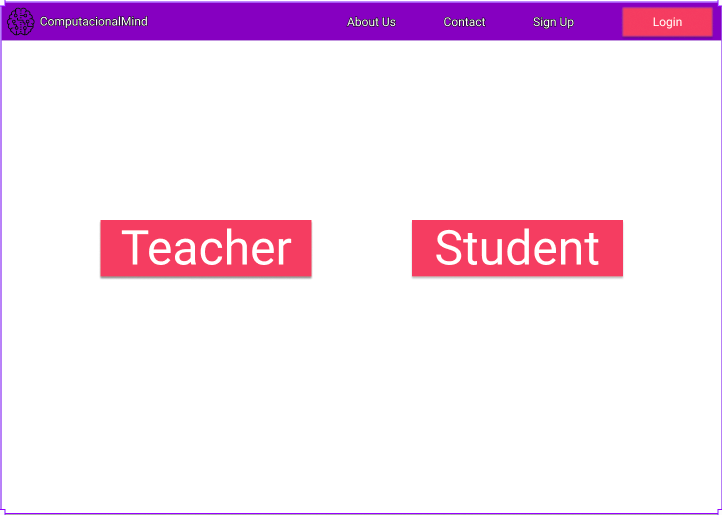
\includegraphics[width=\textwidth]{MockHome.png}
         \caption{Página Principal}
         \label{fig:MockHome}
     \end{subfigure}
     \hfill
     \begin{subfigure}[h!]{0.4\textwidth}
         \centering
         \includegraphics[width=\textwidth]{MockLogin.png}
         \caption{Página de Login}
         \label{fig:MockLogin}
     \end{subfigure}
\end{figure}

\begin{figure}
     \centering
     %\begin{subfigure}[h!]{0.4\linewidth} Outra forma
     \begin{subfigure}[b]{0.4\textwidth}
         \centering
         %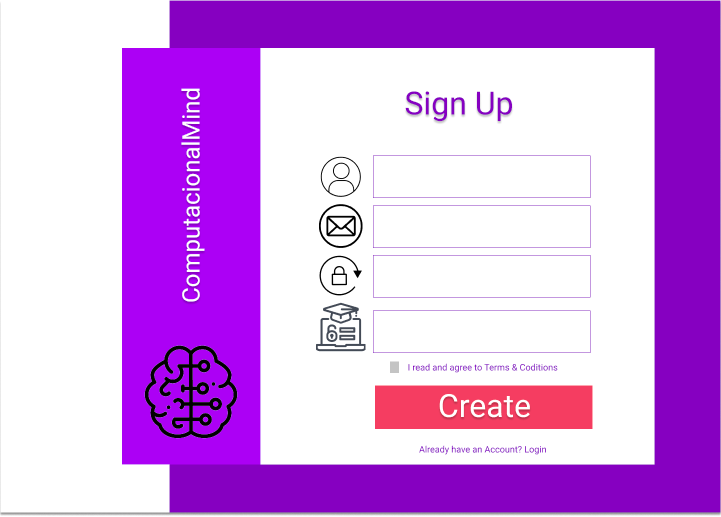
\includegraphics[width=\linewidth]{MockSingUp.png} Outra forma
         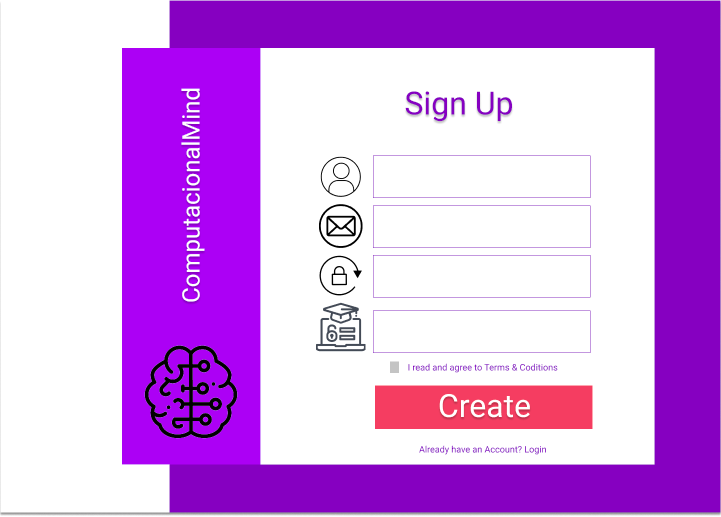
\includegraphics[width=\textwidth]{MockSingUp.png}
         \caption{Página de Criação de Conta}
         \label{fig:MockSingUp}
     \end{subfigure}
     \hfill
     \begin{subfigure}[b]{0.4\textwidth}
         \centering
         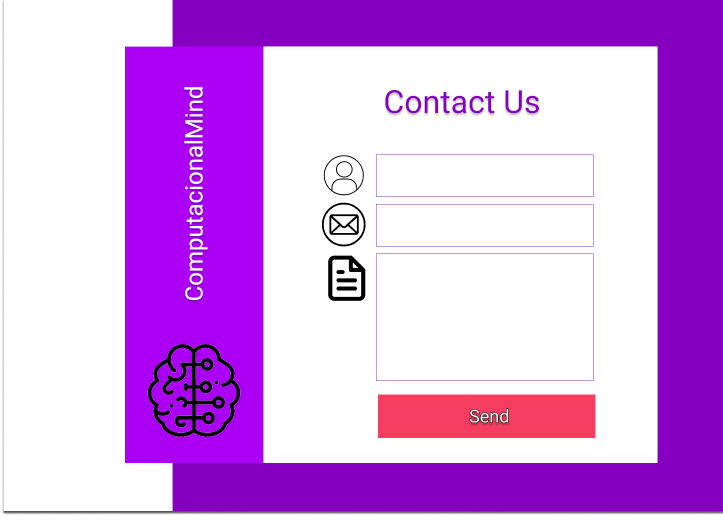
\includegraphics[width=\textwidth]{MockContactUs.png}
         \caption{Página de Contacto}
         \label{fig:MockContactUs}
     \end{subfigure}
     \hfill
     \begin{subfigure}[b]{0.4\textwidth}
         \centering
         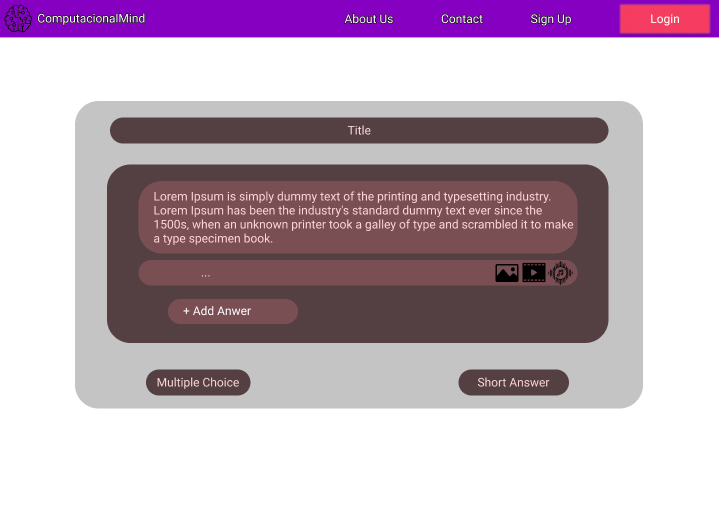
\includegraphics[width=\textwidth]{MockTeacherMenu.png}
         \caption{Menu de Inserção de Jogo}
         \label{fig:MockTeacherMenu}
     \end{subfigure}
     \hfill
     \begin{subfigure}[b]{0.4\textwidth}
         \centering
         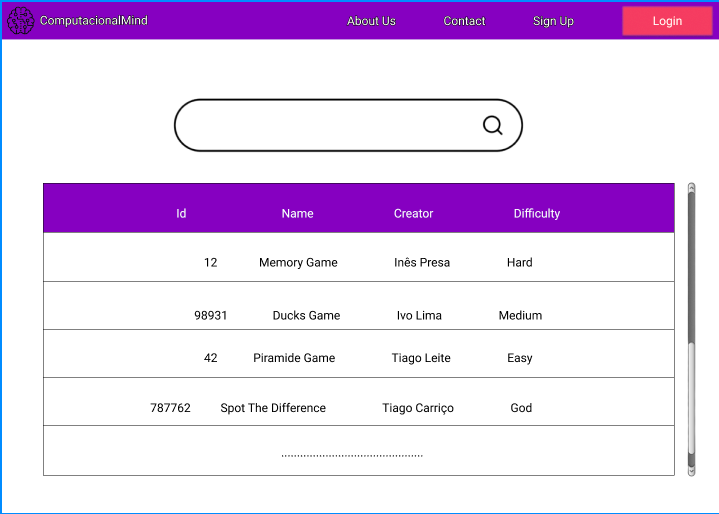
\includegraphics[width=\textwidth]{MockUserSelectGame.png}
         \caption{Menu de Seleção de Jogo}
         \label{fig:MockUserSelectGame}
     \end{subfigure}
     \hfill
     \begin{subfigure}[b]{0.4\textwidth}
         \centering
         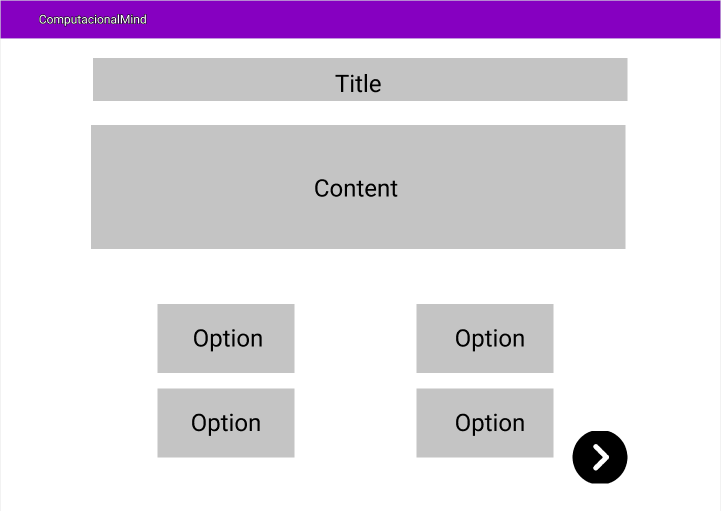
\includegraphics[width=\textwidth]{MockUserGameMC.png}
         \caption{Jogo de Escolha Múltipla}
         \label{fig:MockUserGameMC}
     \end{subfigure}
     \hfill
     \begin{subfigure}[b]{0.4\textwidth}
         \centering
         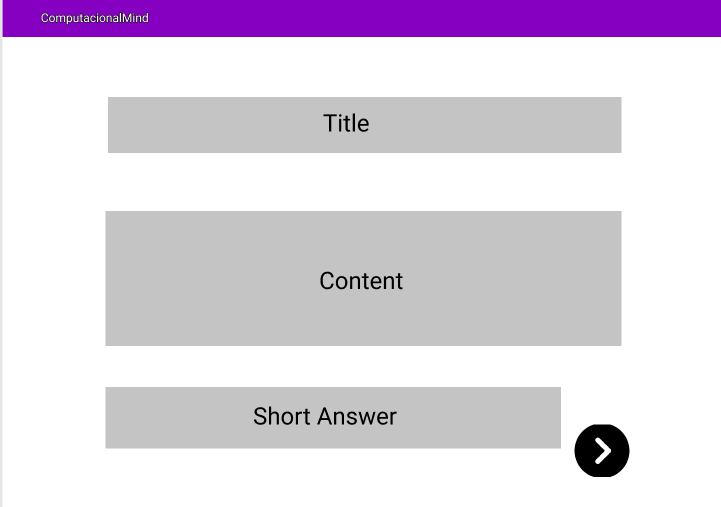
\includegraphics[width=\textwidth]{MockUserGameSA.png}
         \caption{Jogo de Resposta Curta}
         \label{fig:MockUserGameSA}
     \end{subfigure}
\end{figure}

\begin{figure}
    \begin{subfigure}[h]{0.5\linewidth}
        
\includegraphics[width=\linewidth]{MockUserCongratulations.png}
        \caption{Resposta certa}
        \label{fig:MockUserCongratulations}
    \end{subfigure}
    \begin{subfigure}[h]{0.5\linewidth}
        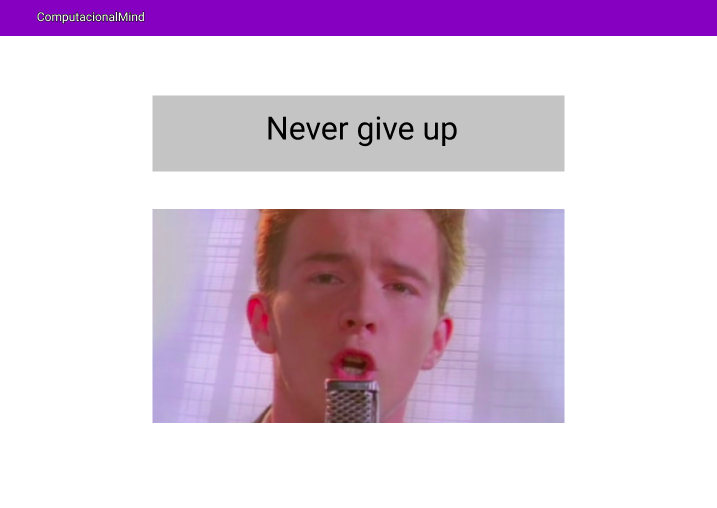
\includegraphics[width=\linewidth]{MockUserTryAgain.png}
        \caption{Resposta errada}
        \label{fig:MockUserTryAgain}
    \end{subfigure}
\end{figure}

\chapter{Base de Dados}

Para este projeto decidimos implementar uma Base de Dados Relacional que permita analisar e relacionar os dados do \emph{Computational Mind} com vista a melhor o serviço, uma vez que esta deverá possibilitar a manipulação e consulta dos dados de uma forma ágil e segura. 
Este será um processo trabalhoso, mas que trará grandes frutos no futuro, uma vez que será substancialmente mais eficiente, especialmente na atualização, consulta e tratamento dos dados, o que permitirá alcançar todos os objetivos propostos pela equipa docente. Para além disso, será também um sistema mais fiável, visto que garantirá uma uniformização dos dados, garantindo que qualquer interveniente que pretenda consultar ou alterar os dados o fará de uma forma mais segura e controlada.

\section{Identificação e caracterização das entidades}

\subsection{Author}
Um autor é identificado por um \textbf{código}, devendo ter também uma referência do seu \textbf{nome}, do \textbf{\emph{e-mail}} e da \textbf{\emph{password}}.

\subsection{Player}
Um jogador é identificado por um \textbf{código}, devendo ter também uma referência do seu \textbf{nome}, da \textbf{data de aniversário}, do \textbf{\emph{e-mail}} e da \textbf{\emph{password}}.

\subsection{Question}
Uma questão é identificado por um \textbf{código}, devendo ter também uma referência ao \textbf{autor}, um \textbf{título}, um identificador do \textbf{tipo} (resposta curta, escolha múltipla ou verdadeiro e falso), uma \textbf{classificação}, a \textbf{dificuldade} e a \textbf{idade mínima}.

\subsection{Content}
Um conteúdo é identificado por uma referência à \textbf{questão}, uma \textbf{ordem} pela qual as questões aparecem, o \textbf{tipo} do conteúdo e os \textbf{links/imagens/vídeos} associados. 

\subsection{Option}
Uma opção é identificada por um \textbf{código}, uma referência à \textbf{questão}, a \textbf{resposta} para serem feitas as verificações e a \textbf{opção correta}.

\subsection{History}
Um histórico é identificado por \textbf{código}, uma referência ao \textbf{jogador}, uma referência à \textbf{questão}, a \textbf{data} que o jogador respondeu à questão, as suas \textbf{respostas} e quais \textbf{acertou}.

\section{Identificação e caracterização dos relacionamentos}

\begin{center}
\begin{tabular}{ |c|c|c|c|c| } 
 \hline
 \bf{Entidade} & \bf{Multiplicidade} & \bf{Relacionamento} & \bf{Multiplicidade} & \bf{Entidade} \\ 
 \hline
 Question & 1..N & tem & 1 & Author \\ 
 \hline
 Option & 1..N & tem & 1 & Question \\ 
 \hline
 History & 1..N & tem & 1 & Question \\ 
 \hline
 History & 1..N & tem & 1 & Player \\ 
 \hline
 Content & 1..N & tem & 1 & Question \\ 
 \hline
\end{tabular}
\end{center}

\section{Modelo lógico}

\begin{figure}[h]
\centering
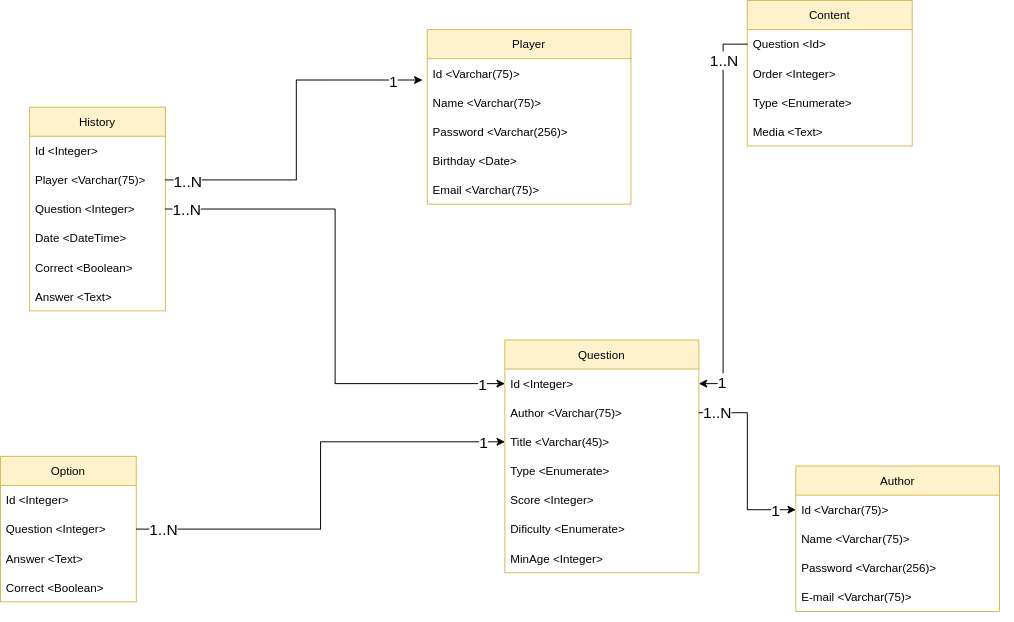
\includegraphics[width = 14cm,height = 10cm]{EsqLog.png}
\caption{Esquema lógico}
\label{fig:EsqLog}
\end{figure}

\section{Alterações}

Por forma a acrescentar  mais funcionalidade e também devido as restrições no desenvolvimento do \emph{back-end}, foram realizadas algumas alterações no modelo inicial da Base de Dados.

\subsection{User}
As entidades \emph{Author} e \emph{Player} passam a ser a entidade \emph{User} que tem um atributo \emph{type} para fazer a distinção entre ambos.

\subsection{Quiz}
Um quiz é constituído por várias questões. É identificado através de um \textbf{código}, devendo ter ainda uma referência ao \textbf{autor} e um \textbf{título}.

\subsection{Identificação e caracterização dos relacionamentos}

\begin{center}
\begin{tabular}{ |c|c|c|c|c| } 
 \hline
 \bf{Entidade} & \bf{Multiplicidade} & \bf{Relacionamento} & \bf{Multiplicidade} & \bf{Entidade} \\ 
 \hline
 Quiz & 1..N & tem & 1 & User \\ 
 \hline
 Question & 1..N & tem & 1 & User \\ 
 \hline
 Question & 1..N & tem & 1 & Quiz \\ 
 \hline
 Option & 1..N & tem & 1 & Question \\ 
 \hline
 History & 1..N & tem & 1 & Question \\ 
 \hline
 History & 1..N & tem & 1 & User \\ 
 \hline
 Content & 1..N & tem & 1 & Question \\ 
 \hline
\end{tabular}
\end{center}

\subsection{Modelo lógico final}

\begin{figure}[h]
\centering
\includegraphics[width = 12cm,height = 8cm]{EsqLogFin.png}
\caption{Esquema lógico final}
\label{fig:EsqLogFini}
\end{figure}

\chapter{Back-end}

\section{Ferramentas}

Para o desenvolvimento da  \emph{parte secundária} utilizou-se \emph{Django} e \emph{Django REST Framework}.

\section{Django}

\emph{Django} é uma \emph{framework} gratuita e de código aberto, com o intuito de facilitar e acelerar o desenvolvimento \emph{web}, escrito em Python, que utiliza o padrão \emph{model-template-view} (MTV) e o princípio \emph{don't repeat yourself} (DRY) através do reaproveitamento de código já feito. O \emph{web\ server}, pode ajudar os \emph{developers} a produzir de forma eficiente um FO ou BO rico em recursos, seguro e escalável.

O \emph{Django REST Framework} é um conjunto de ferramentas utilizadas para construir \emph{APIs} (Interfaces de Programação de Aplicações) para \emph{Web}.

Apesar do \emph{Django} possibilitar o desenvolvimento do \emph{front-end} e do \emph{back-end}, a utilização de uma \emph{REST API} permite criar uma \emph{parte de suporte} mais genérica, e torna possível a construção de uma \emph{parte frontal} para diversos dispositivos no futuro, tornando a nossa aplicação mais escalável. 

\section{Objetivo}

O \emph{back-end} do projeto tem como objetivo fazer a ligação entre a Base de Dados e a \emph{interface frontal}, tendo sido desenvolvido ainda uma \emph{REST API} que será "consumida" pela mesma.
\newpage
\section{Desenvolvimento}
O processo de desenvolvimento começou pela construção da base de dados através do \emph{Django}, com base no esquema lógico definido. Para tal, foram construídos todos os modelos necessários para representar as várias entidades e os seus relacionamentos. A construção da base de dados foi feita com recurso à funcionalidade \emph{migrate} disponibilizada pelo \emph{Django}. O sistema de gestão de base de dados utilizado foi o \emph{MySQL}.
Devido a algumas restrições imposta pelo \emph{Django}, foi necessário realizar algumas alterações no esquema lógico, inicialmente, definido.

A principal função do \emph{Django} é servir de intermediário da comunicação entre a \emph{parte frontal} e a base de dados. Essa comunicação é realizada através da \emph{REST API} com o envio de ficheiros em formato \emph{JSON}. Para tal, o \emph{Django} possui funções específicas para serializar os dados. 

A comunicação entre os constituintes desta plataforma ocorre da seguinte forma: 
\begin{enumerate}
    \item O \emph{ReactJs} faz uma pedido através da \emph{REST API}.
    \item Este pedido é analisado \emph{Django} e, caso esteja correto, os dados requeridos são extraídos da base de dados, convertidos e enviados para a \emph{interface frontal} no formato \emph{JSON}.
\end{enumerate}

É de destacar que a comunicação inversa é também possível e processa-se de modo análogo.
\newline\newline

\begin{figure}[h]
\centering
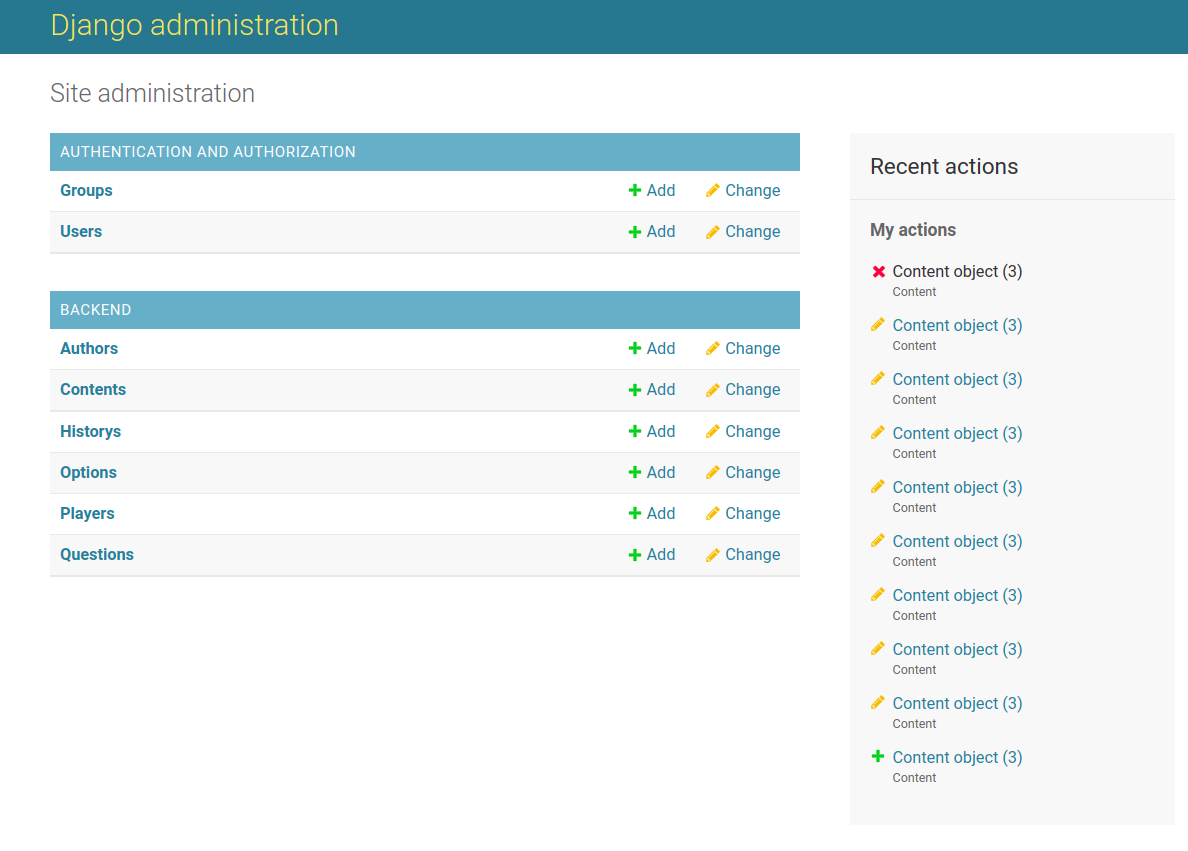
\includegraphics[width = 14cm,height = 10cm]{apiDjango.png}
\caption{REST API}
\label{fig:pagDJang}
\end{figure}

\newpage

\section{Manual da API}

\subsection{/api/profile/}

\textbf{tipo:} GET.

\textbf{função:} obter dados do \emph{user} que está autenticado.

\textbf{requisitos:} autenticação.

\textbf{resposta:}

\begin{lstlisting}[style = code]
    {
        "id": 9,
        "username": "username",
        "name": "name",
        "birthday": null,
        "email": "email@email.com",
        "type": "A"
    }
\end{lstlisting}

\textbf{status correto}: 200.

\textbf{status errado}: 401.

\subsection{/api/profile/password/}

\textbf{tipo:} POST.

\textbf{função:} alterar a \emph{password} do \emph{user} que está autenticado.

\textbf{requisitos:} autenticação.

\textbf{pedido:}

\begin{lstlisting}[style = code]
   {
        "current":"0123",
        "new":"56789"
    }
\end{lstlisting}

\textbf{status correto}: 200.

\textbf{status errado}: 403.

\newpage

\subsection{/api/users/}

\textbf{tipo:} POST.

\textbf{função:} alterar a \emph{password} do \emph{user} que está autenticado.

\textbf{requisitos:} autenticação.

\textbf{pedido:}

\begin{lstlisting}[style = code]
   {
        "username": "username",
        "name": "name",
        "password": "password",
        "email": "email@email.com",
        "birthday": null,
        "type": "A"
    }
\end{lstlisting}

\textbf{status correto}: 200.

\textbf{status errado}: 403.


\subsection{/api/users/$<$str:username$>$}

\textbf{tipo:} GET.

\textbf{função:} obter a informação do \emph{user} que esta autenticado e com \emph{usernanme} = $<$str:username$>$

\textbf{requisitos:} autenticação.

\textbf{resposta:}

\begin{lstlisting}[style = code]
   {
        "id": 1,
        "username": "username",
        "name": "name",
        "birthday": null,
        "email": "email@email.com",
        "type": "A"
    }
\end{lstlisting}

\textbf{status correto}: 200.

\textbf{status errado}: 404.

\newpage

\subsection{/api/questions/}

\textbf{tipo:} GET.

\textbf{função:} obter todas as questões.

\textbf{requisitos:} autenticação.

\textbf{resposta:}

\begin{lstlisting}[style = code]
    [
        {
            "id": 1,
            "author": "username",
            "title": "Teste",
            "type": "SA",
            "score": 10,
            "dificulty": "E",
            "minage": 5,
            "options": [
                {
                    "id": 1,
                    "answer": "Ola Mundo",
                    "question": 1,
                    "correct": true
                },
                {
                    "id": 2,
                    "answer": "Mundo",
                    "question": 1,
                    "correct": false
                }
            ],
            "contents": [
                {
                    "id": 1,
                    "question": 1,
                    "order": 1,
                    "type": "T",
                    "text": "Escreva Ola Mundo",
                    "media": null
                }
            ],
            "quiz": 1
        }
    ]
\end{lstlisting}

\textbf{status correto}: 200.

\textbf{status errado}: 401.

\textbf{Nota:} Se o \emph{user} que faz o pedido for do tipo \emph{P} o campo \emph{correct} nas \emph{options} é removido.

\newpage

\subsection{/api/questions/$<$int:id$>$}

\textbf{tipo:} GET.

\textbf{função:} obter a questão com \emph{id} = $<$int:id$>$.

\textbf{requisitos:} autenticação.

\textbf{resposta:}

\begin{lstlisting}[style = code]
    {
        "id": 1,
        "author": "username",
        "title": "Teste",
        "type": "SA",
        "score": 10,
        "dificulty": "E",
        "minage": 5,
        "options": [
            {
                "id": 1,
                "answer": "Ola Mundo",
                "question": 1,
                "correct": true
            },
            {
                "id": 2,
                "answer": "Mundo",
                "question": 1,
                "correct": false
            }
        ],
        "contents": [
            {
                "id": 1,
                "question": 1,
                "order": 1,
                "type": "T",
                "text": "Escreve Ola Mundo",
                "media": null
            }
        ],
        "quiz": 1
    }
    
\end{lstlisting}

\textbf{status correto}: 200.

\textbf{status errado}: 401.

\textbf{Nota:} Se o \emph{user} que faz o pedido for do tipo \emph{P} o campo \emph{correct} nas \emph{options} é removido.

\newpage

\subsection{/api/questions/user/}

\textbf{tipo:} GET.

\textbf{função:} obter todas as questões do autor autenticado.

\textbf{requisitos:} autenticação.

\textbf{resposta:}

\begin{lstlisting}[style = code]
   [
        {
            "id": 1,
            "author": "username",
            "title": "Teste",
            "type": "SA",
            "score": 10,
            "dificulty": "E",
            "minage": 5,
            "options": [
                {
                    "id": 1,
                    "answer": "Ola Mundo",
                    "question": 1,
                    "correct": true
                },
                {
                    "id": 2,
                    "answer": "Mundo",
                    "question": 1,
                    "correct": false
                }
            ],
            "contents": [
                {
                    "id": 1,
                    "question": 1,
                    "order": 1,
                    "type": "T",
                    "text": "Escreve Ola Mundo",
                    "media": null
                }
            ],
        }"quiz": 1
    ]
    
\end{lstlisting}

\textbf{status correto}: 200.

\textbf{status errado}: 401.

\newpage

\subsection{/api/questions/insert/}

\textbf{tipo:} POST.

\textbf{função:} inserir uma questão

\textbf{requisitos:} autenticação e ser um \emph{user} do tipo \emph{author}

\textbf{pedido:}

\begin{lstlisting}[style = code]
   {
        "title": "title",
        "type": "SA",
        "score": 10,
        "dificulty": "E",
        "minage": 5,
        "options": [
            {
                "answer": "Ola Mundo",
                "correct": true
            }
        ],
        "contents": [
            {
                "order": 1,
                "type": "T",
                "text": "Escreva Ola Mundo"
            }
        ]
    }
\end{lstlisting}

\textbf{resposta:}

\begin{lstlisting}[style = code]
   {
    	"id": 1,
    	"author": 1,
    	"title": "title",
    	"type": "SA",
    	"score": 10,
    	"dificulty": "E",
    	"minage": 5,
    	"options": [
    		{
    			"id": 1,
    			"answer": "Ola Mundo",
    			"question": 1,
    			"correct": true
    		}
    	],
    	"contents": [
    		{
    			"id": 1,
    			"question": 1,
    			"order": 1,
    			"type": "T",
    			"text": "Escreva Ola Mundo",
    			"media": null
    		}
    	],
    	"quiz": null
}
\end{lstlisting}

\textbf{status correto}: 201.

\textbf{status errado}: 401 ou 403.

\subsection{/api/questions/update/$<$int:id$>$}

\textbf{tipo:} POST.

\textbf{função:} alterar a questão com \emph{id} = $<$int:id$>$

\textbf{requisitos:} autenticação e ser o autor da questão.

\textbf{pedido:}

\begin{lstlisting}[style = code]
   {
        "title": "title",
        "type": "SA",
        "score": 10,
        "dificulty": "E",
        "minage": 5,
        "options": [
            {
                "id": 1,
                "answer": "Ola",
                "correct": true
            }
        ],
        "contents": [
            {
                "id":1,
                "order": 1,
                "type": "T",
                "text": "Escreva Ola"
            }
        ]
    }
\end{lstlisting}

\textbf{resposta:}

\begin{lstlisting}[style = code]
{
        "id":
        "title": "title",
        "type": "SA",
        "score": 10,
        "dificulty": "E",
        "minage": 5,
        "options": [
            {
                "id": 1,
                "answer": "Ola",
                "correct": true
            }
        ],
        "contents": [
            {
                "id":1,
                "order": 1,
                "type": "T",
                "text": "Escreva Ola",
                "media" null
            }
        ],
        "quiz": null
    }
\end{lstlisting}

\textbf{Status correto}: 200.

\textbf{Status errado}: 403 ou 404.

\textbf{nota:} os campos que não forem enviado serão mantidos. Só serão mantidas as \emph{options} e \text{questions} para as quais seja enviado o seu \emph{id}. Se não for enviado o \emph{id}, serão criadas novas instâncias. 

\subsection{/api/questions/delete/$<$int:id$>$}

\textbf{tipo:} POST.

\textbf{função:} apagar a questão com \emph{id} = $<$int:id$>$

\textbf{requisitos:} autenticação e ser o autor da questão.

\textbf{status correto}: 200.

\textbf{status errado}: 403 ou 404.


\subsection{/api/quizzes/}

\textbf{tipo:} GET.

\textbf{função:} obter todos os quizzes.

\textbf{requisitos:} autenticação.

\textbf{resposta:}

\begin{lstlisting}[style = code]
    [{
		"id": 1,
		"questions": [
			{
                "id":
                "title": "title",
                "type": "SA",
                "score": 10,
                "dificulty": "E",
                "minage": 5,
        "options": [
            {
                "id": 1,
                "answer": "Ola",
                "correct": true
            }
        ],
        "contents": [
            {
                "id":1,
                "order": 1,
                "type": "T",
                "text": "Escreva Ola",
                "media" null
            }
        ],
        "quiz": 1
        }], 
	    "author": 1,
	    "title": "quiz"
    }]
\end{lstlisting}

\textbf{status correto}: 200.

\textbf{status errado}: 401.

\textbf{Nota:} Se o \emph{user} que faz o pedido for do tipo \emph{P} o campo \emph{correct} nas \emph{options} de cada questão é removido.



\subsection{/api/quizzes/$<$int:id$>$}

\textbf{tipo:} GET.

\textbf{função:} obter o quiz com \emph{id} = $<$int:id$>$.

\textbf{requisitos:} autenticação.

\textbf{resposta:}

\begin{lstlisting}[style = code]
    {
		"id": 1,
		"questions": [
			{
                "id":
                "title": "title",
                "type": "SA",
                "score": 10,
                "dificulty": "E",
                "minage": 5,
        "options": [
            {
                "id": 1,
                "answer": "Ola",
                "correct": true
            }
        ],
        "contents": [
            {
                "id":1,
                "order": 1,
                "type": "T",
                "text": "Escreva Ola",
                "media" null
            }
        ],
        "quiz": 1
        }], 
	    "author": 1,
	    "title": "quiz"
    }
\end{lstlisting}

\textbf{status correto}: 200.

\textbf{status errado}: 401 ou 404.

\textbf{Nota:} Se o \emph{user} que faz o pedido for do tipo \emph{P} o campo \emph{correct} nas \emph{options} de cada questão é removido.

\subsection{/api/quizzes/user/}

\textbf{tipo:} GET.

\textbf{função:} obter todos os quizzes do autor autenticado.

\textbf{requisitos:} autenticação.

\textbf{resposta:}

\begin{lstlisting}[style = code]
    [{
		"id": 1,
		"questions": [
			{
                "id":
                "title": "title",
                "type": "SA",
                "score": 10,
                "dificulty": "E",
                "minage": 5,
        "options": [
            {
                "id": 1,
                "answer": "Ola",
                "correct": true
            }
        ],
        "contents": [
            {
                "id":1,
                "order": 1,
                "type": "T",
                "text": "Escreva Ola",
                "media" null
            }
        ],
        "quiz": 1
        }], 
	    "author": 1,
	    "title": "quiz"
    }]
\end{lstlisting}

\textbf{status correto}: 200.

\textbf{status errado}: 401.

\newpage

\subsection{/api/quizzes/insert/}

\textbf{tipo:} POST.

\textbf{função:} inserir um quiz

\textbf{requisitos:} autenticação e ser um \emph{user} do tipo \emph{author}

\textbf{pedido:}

\begin{lstlisting}[style = code]
    {
		"questions": [
			{
                "title": "title",
                "type": "SA",
                "score": 10,
                "dificulty": "E",
                "minage": 5,
        "options": [
            {
                "answer": "Ola Mundo",
                "correct": true
            }
    ],
        "contents": [
            {
                "order": 1,
                "type": "T",
                "text": "Escreva Ola Mundo"
            }
        ]
        }],
        "title": "quiz"
    }
\end{lstlisting}

\textbf{resposta:}

\begin{lstlisting}[style = code]
{
	"id": 1,
	"questions": [
		{
			"id": 1,
			"author": 1,
			"title": "title",
			"type": "SA",
			"score": 10,
			"dificulty": "E",
			"minage": 5,
			"options": [
				{
					"id": 1,
					"answer": "Ola Mundo",
					"question": 134,
					"correct": true
				}
			],
			"contents": [
				{
					"id": 1,
					"question": 1,
					"order": 1,
					"type": "T",
					"text": "Escreva Ola Mundo",
					"media": null
				}
			],
			"quiz": 1
		}
	],
	"author": 1,
	"title": "quiz"
}
\end{lstlisting}

\textbf{status correto}: 201.

\textbf{status errado}: 401 ou 403.


\subsection{/api/quizzes/update/$<$int:id$>$}

\textbf{tipo:} POST.

\textbf{função:} alterar o quiz com \emph{id} = $<$int:id$>$

\textbf{requisitos:} autenticação e ser o autor do quiz.

\textbf{pedido:}

\begin{lstlisting}[style = code]
   {
	"questions": [
		{
			"id":1,
			"author": 1,
			"title": "title",
			"type": "SA",
			"score": 10,
			"dificulty": "E",
			"minage": 5,
			"options": [
				{
					"id":1,
					"answer": "Ola",
					"correct": true
				}
			],
			"contents": [
				{
					"id":1,
					"order": 1,
					"type": "T",
					"text": "Escreva Ola"
					
				}
			]
	
		}
	]
}
\end{lstlisting}

\textbf{resposta:}

\begin{lstlisting}[style = code]
{
	"id": 1,
	"questions": [
		{
			"id": 1,
			"author": 1,
			"title": "title",
			"type": "SA",
			"score": 10,
			"dificulty": "E",
			"minage": 5,
			"options": [
				{
					"id": 223,
					"answer": "Ola",
					"question": 211,
					"correct": true
				}
			],
			"contents": [
				{
					"id": 1,
					"question": 1,
					"order": 1,
					"type": "T",
					"text": "Escreva Ola",
					"media": null
				}
			],
			"quiz": 1
		}
	],
	"author": 1,
	"title": "quiz"
}
\end{lstlisting}

\textbf{Status correto}: 200.

\textbf{Status errado}: 403 ou 404.

\subsection{/api/quizzes/delete/$<$int:id$>$}

\textbf{tipo:} POST.

\textbf{função:} apagar o quiz com \emph{id} = $<$int:id$>$

\textbf{requisitos:} autenticação e ser o autor do quiz.

\textbf{status correto}: 200.

\textbf{status errado}: 403 ou 404.

\newpage

\subsection{/api/history/}

\textbf{tipo:} POST.

\textbf{função:} inserir a resposta a uma questão.

\textbf{requisitos:} autenticação e o \emph{user} ser do tipo \emph{Player}.

\textbf{pedido:}
\begin{lstlisting}[style = code]
    {
        "question": "1",
        "answer": "Ola"
    }
\end{lstlisting}

\textbf{resposta:}

\begin{lstlisting}[style = code]
    {
        "id": 1,
        "player": 2,
        "question": 1,
        "date": "2022-06-27T01:09:23Z",
        "correct": true,
        "answer": "Ola"
    }
\end{lstlisting}

\textbf{status correto}: 201.

\textbf{status errado}: 401 ou 404.

\newpage

\subsection{/api/history/user/}

\textbf{tipo:} GET.

\textbf{função:} obter o historio de respostas do utilizador que está autenticado.

\textbf{requisitos:} autenticação e o \emph{user} ser do tipo \emph{Player}.

\textbf{pedido:}
\begin{lstlisting}[style = code]
    {
        "question": "1",
        "answer": "ola"
    }
\end{lstlisting}

\textbf{resposta:}

\begin{lstlisting}[style = code]
    [
        {
            "id": 1,
            "player": "2",
            "question": 1,
            "date": "2022-06-27T01:09:23Z",
            "correct": true,
            "answer": "Ola"
        },
        {
            "id": 2,
            "player": "2",
            "question": 2,
            "date": "2022-06-26T22:02:10Z",
            "correct": true,
            "answer": "mundo"
        }
]
\end{lstlisting}

\textbf{status correto}: 200.

\textbf{status errado}: 401.

\newpage

\subsection{/api/history/question/$<$int:id$>$}

\textbf{tipo:} GET.

\textbf{função:} obter o historio de respostas da questão com \emph{id} = $<$int:id$>$.

\textbf{requisitos:} autenticação e ser o autor da questão.

\textbf{resposta:}

\begin{lstlisting}[style = code]
    [
        {
            "id": 1,
            "player": "2",
            "question": 1,
            "date": "2022-06-27T01:09:23Z",
            "correct": true,
            "answer": "Ola"
        }
]
\end{lstlisting}

\textbf{status correto}: 200.

\textbf{status errado}: 401 ou 404.

\subsection{/api/login/}

\textbf{tipo:} POST.

\textbf{função:} autenticar um \emph{user}.


\textbf{pedido:}

\begin{lstlisting}[style = code]
    {
        "username": "username",
        "password":"password"
    }
\end{lstlisting}

\emph{resposta:}

\begin{lstlisting}[style = code]
    {
        "refresh": "eyJ0eXAiOiJKV1QiLCJhbGciOiJIUzI1NiJ9.
        eyJ0b2tlbl90eXBlIjoicmVmcmVzaCIsImV4cCI6MTY1NjM3
        ODUzMiwiaWF0IjoxNjU2MjkyMTMyLCJqdGkiOiIyMjFjZjAz
        YWUxODE0Nzc5ODI3NjNmOWMxOGYwYjY1MyIsInVzZXJfaWQiOjl9.
        8Qlwm7xgbjZFEH0ndK7CiNS1P-D4FCoRnPb4jLf7-Io",
    
        "access": "eyJ0eXAiOiJKV1QiLCJhbGciOiJIUzI1NiJ9.
        eyJ0b2tlbl90eXBlIjoiYWNjZXNzIiwiZXhwIjoxNjU2Mjk1Nz
        MyLCJpYXQiOjE2NTYyOTIxMzIsImp0aSI6IjdlMTM3OTE5OWM1
        OTQ3NWViODFmMGQ2Y2MyMWU1OTFkIiwidXNlcl9pZCI6OX0.
        TDjrl61WosT_hMp1UMCOCI-iG3DZnU93QKuu3aIAVho"
    }

\end{lstlisting}

\textbf{status correto}: 200.

\textbf{status errado}: 401.

\newpage

\subsection{/api/login/refresh/}

\textbf{tipo:} POST.

\textbf{função:} atualizar o \emph{token} quando expirado.

\textbf{pedido:}

\begin{lstlisting}[style = code]
    {
        "refresh":"eyJ0eXAiOiJKV1QiLCJhbGciOiJIUzI1NiJ9.
        eyJ0b2tlbl90eXBlIjoicmVmcmVzaCIsImV4cCI6MTY1NjM3O
        TY4OSwiaWF0IjoxNjU2MjkzMjg5LCJqdGkiOiI2ZDcwMjQ5N2
        VjYTE0ZmQ0YjQzMjM5YzMzNDQ5NjNiMiIsInVzZXJfaWQiOjl9.
        0lB2EG0DjDjIiZt2OqBuUjy1Zw8c71uCOHf-UMTHY2I"  
    }
\end{lstlisting}

\emph{resposta:}

\begin{lstlisting}[style = code]
    {
        "access": "eyJ0eXAiOiJKV1QiLCJhbGciOiJIUzI1NiJ9.
        eyJ0b2tlbl90eXBlIjoiYWNjZXNzIiwiZXhwIjoxNjU2Mjk3N
        DQxLCJpYXQiOjE2NTYyOTMyODksImp0aSI6ImY1YjNhOWY2ZDY
        zYzRjOWY4Yjc5ZWFkODRkNTJiMzEyIiwidXNlcl9pZCI6OX0.
        SPNTGHdXwGwVod-1VZLSJvRIRo5mIECk6brbTqwOE34"
    }
\end{lstlisting}

\textbf{status correto}: 200.

\textbf{status errado}: 401.

\subsection{/api/login/verify/}

\textbf{tipo:} POST.

\textbf{função:} verificar se o \emph{token} é válido.

\textbf{pedido:}

\begin{lstlisting}[style = code]
    {
        "token":"eyJ0eXAiOiJKV1QiLCJhbGciOiJIUzI1NiJ9.
        eyJ0b2tlbl90eXBlIjoiYWNjZXNzIiwiZXhwIjoxNjU2Mjk2
        ODg5LCJpYXQiOjE2NTYyOTMyODksImp0aSI6Ijg1YzM3YWJi
        OTZjNTQ0Y2U4M2M2ZmY5MzBiMTgwMTdjIiwidXNlcl9pZCI6OX0.
        -C5f3KhAUgN_udTNjgQtTEIYqc80zFmafsjb19nHshc" 
    }
\end{lstlisting}

\emph{resposta:}

\textbf{status correto}: 200.

\textbf{status errado}: 401.

\newpage

\chapter{Front-End}

\section{Ferramentas}
Para o desenvolvimento do  \emph{front-end} utilizou-se \emph{React} e \emph{TailWindCSS}.

\section{React e TailWindCSS}

\emph{React.js} é uma biblioteca \emph{JavaScript} de código aberto usada para construir o \emph{front-end} de aplicativos e de páginas \emph{web} utilizando a lógica de página única. Sendo usada para lidar com a camada de visualização para as aplicações da \emph{Web} e de telemóvel. 

Para além disso, esta também nos permite criar componentes para a interface do usuário que sejam reutilizáveis para que os \emph{developers} criem grandes aplicações, por forma a facilitar a alteração dos dados sem que seja necessário o recarregar a página. O seu principal objetivo é ser rápido, escalável e simples. Este funciona apenas em interfaces de usuário no aplicativo, o que corresponde à exibição do modelo \emph{Model-View-Controller} (MVC), existindo a possibilidade de ser usado em conjunto com outras bibliotecas ou \emph{frameworks} de \emph{JavaScript}, como \emph{Angular\ JS} em MVC.

\emph{Tailwind\ CSS} corresponde, basicamente, a uma \emph{framework} de \emph{CSS} fundamental para a construção rápida de interfaces de utilizador personalizadas. Sendo que uma estrutura \emph{CSS} é altamente personalizável e de baixo nível que fornece todos os blocos de construção necessários para criar \emph{designs} sob medida, sem que seja necessária a escrita de \emph{CSS} como na abordagem tradicional.

\section{Objetivo}

O \emph{front-end} é responsável por possibilitar a interação do utilizador com a página dentro de uma aplicação \emph{web} e cobrindo as questões da política de privacidade.
\newpage
\section{Desenvolvimento}

O desenvolvimento do \emph{front-end} começou com o desenho dos \emph{Mockups} no \emph{Figma}, que serviram como base inicial. No entanto, ao longo deste desenvolvimento, o aspeto do \emph{web site} foi divergindo do, inicialmente, desenhado.

A construção, propriamente dita, do \emph{front-end} realizou-se em \emph{ReactJS}, uma vez que alguns dos elementos do grupo já possuíam conhecimentos na utilização desta \emph{framework}. Relativamente à estilização,  utilizou-se a \emph{framework TailWindCSS}.

O \emph{front-end} é a componente da plataforma com o qual o utilizador interage, sendo da sua responsabilidade receber os pedidos e comunicá-los ao \emph{back-end}. Como a esmagadora maioria dos utilizadores não apresenta conhecimentos ao nível informático, o \emph{front-end} adquire especial importância, dado que se o aspeto da plataforma não for apelativo, por melhor que seja a sua implementação ao nível lógico, esta não será valorizada pelo utilizador, e o site terá pouca adesão.

\chapter{ComputationalMind}

Ao longo deste semestre desenvolvemos a página do \emph{ComputationalMind} até que o produto final fosse semelhante ao que foi idealizado e apresentado nos capítulos anteriores. Em seguida, será demonstrado o funcionamento e onde se podem encontrar todas as funcionalidades implementadas.

\section{Página inicial}

Na página inicial consideramos que o utilizador pode ser um \emph{Player} que apenas usufrui dos jogos disponibilizados na plataforma pelo \emph{Author} que é a entidade que criou o jogo.\newline\newline

\begin{figure}[h]
    \centering
    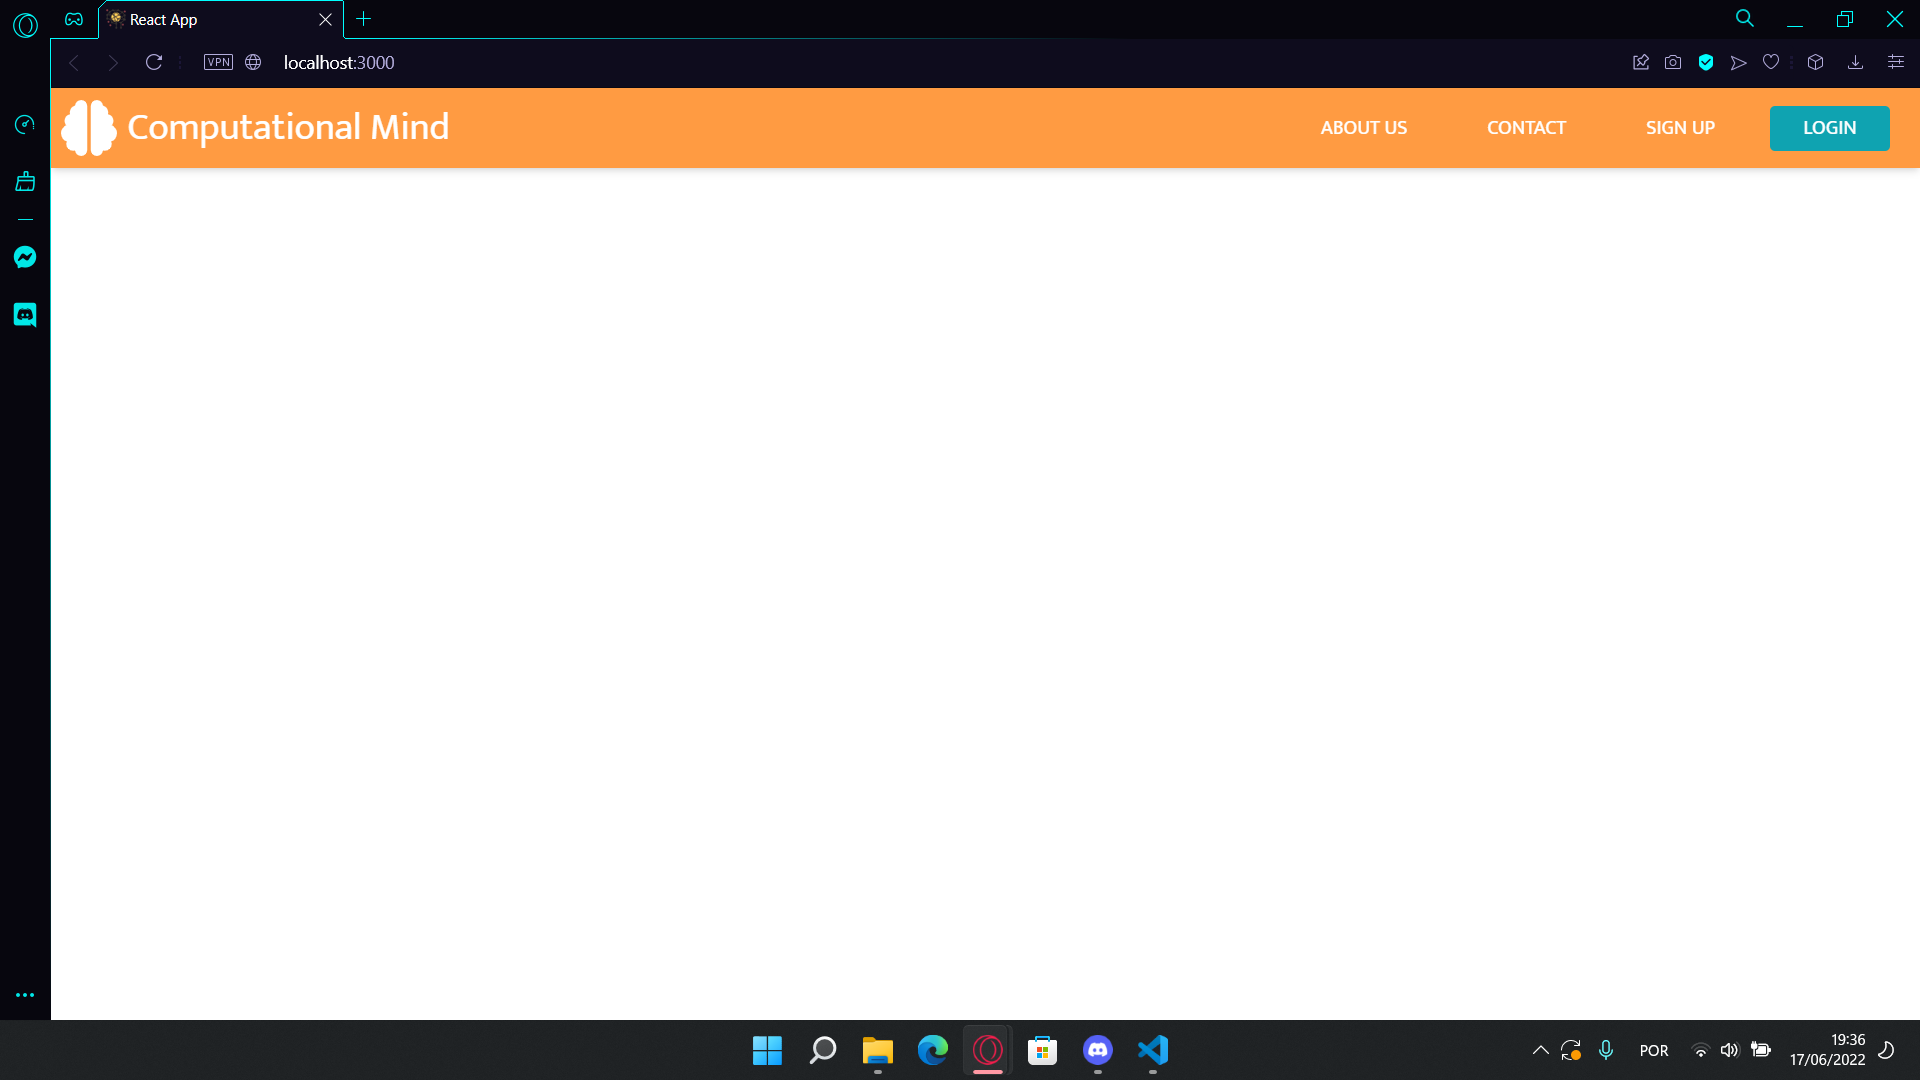
\includegraphics[width = 10cm]{pagIni.png}
    \caption{Página Principal}
    \label{fig:pagIni}
\end{figure}

\newpage

\section{About Us}

Nesta secção incorporamos informação sobre o propósito da página.\newline

\begin{figure}[h]
    \centering
    
\includegraphics[width = 10cm]{aboutUs.png}
    \caption{About Us}
    \label{fig:abUs}
\end{figure}

\section{Contact}

Aqui os utilizadores podem informar os \emph{developers} de possíveis \emph{bugs} que tenham encontrado ou sugerir novas funcionalidades que tornariam a plataforma mais apelativa ou cómoda para quem a usa.

\begin{figure}[h]
    \centering
    \includegraphics[width = 10cm]{contUs.png}
    \caption{Contact}
    \label{fig:cont}
\end{figure}

\newpage

\section{\emph{Login} / \emph{Sign Up}}
Após a escolha de uma das opções disponibilizadas na página inicial, os utilizadores serão redirecionados para a página de \emph{Login} / \emph{Sign Up}. 

Nesta página é possível um utilizador autenticar-se ou efetuar o seu registo no site. 

A página de autentificação é igual para ambos os utilizadores, a única diferença na página de \emph{Sign Up} do \emph{Player Sign Up} para a do \emph{Author Sign Up} é que na do \emph{Player} é relevante saber a idade para serem apresentados jogos mais adequados à sua faixa etária enquanto que na do \emph{Author} essa informação não é relevante.\newline\newline

\begin{figure}[h]%
    \centering
    \subfloat[\centering Página de \emph{Login}]{{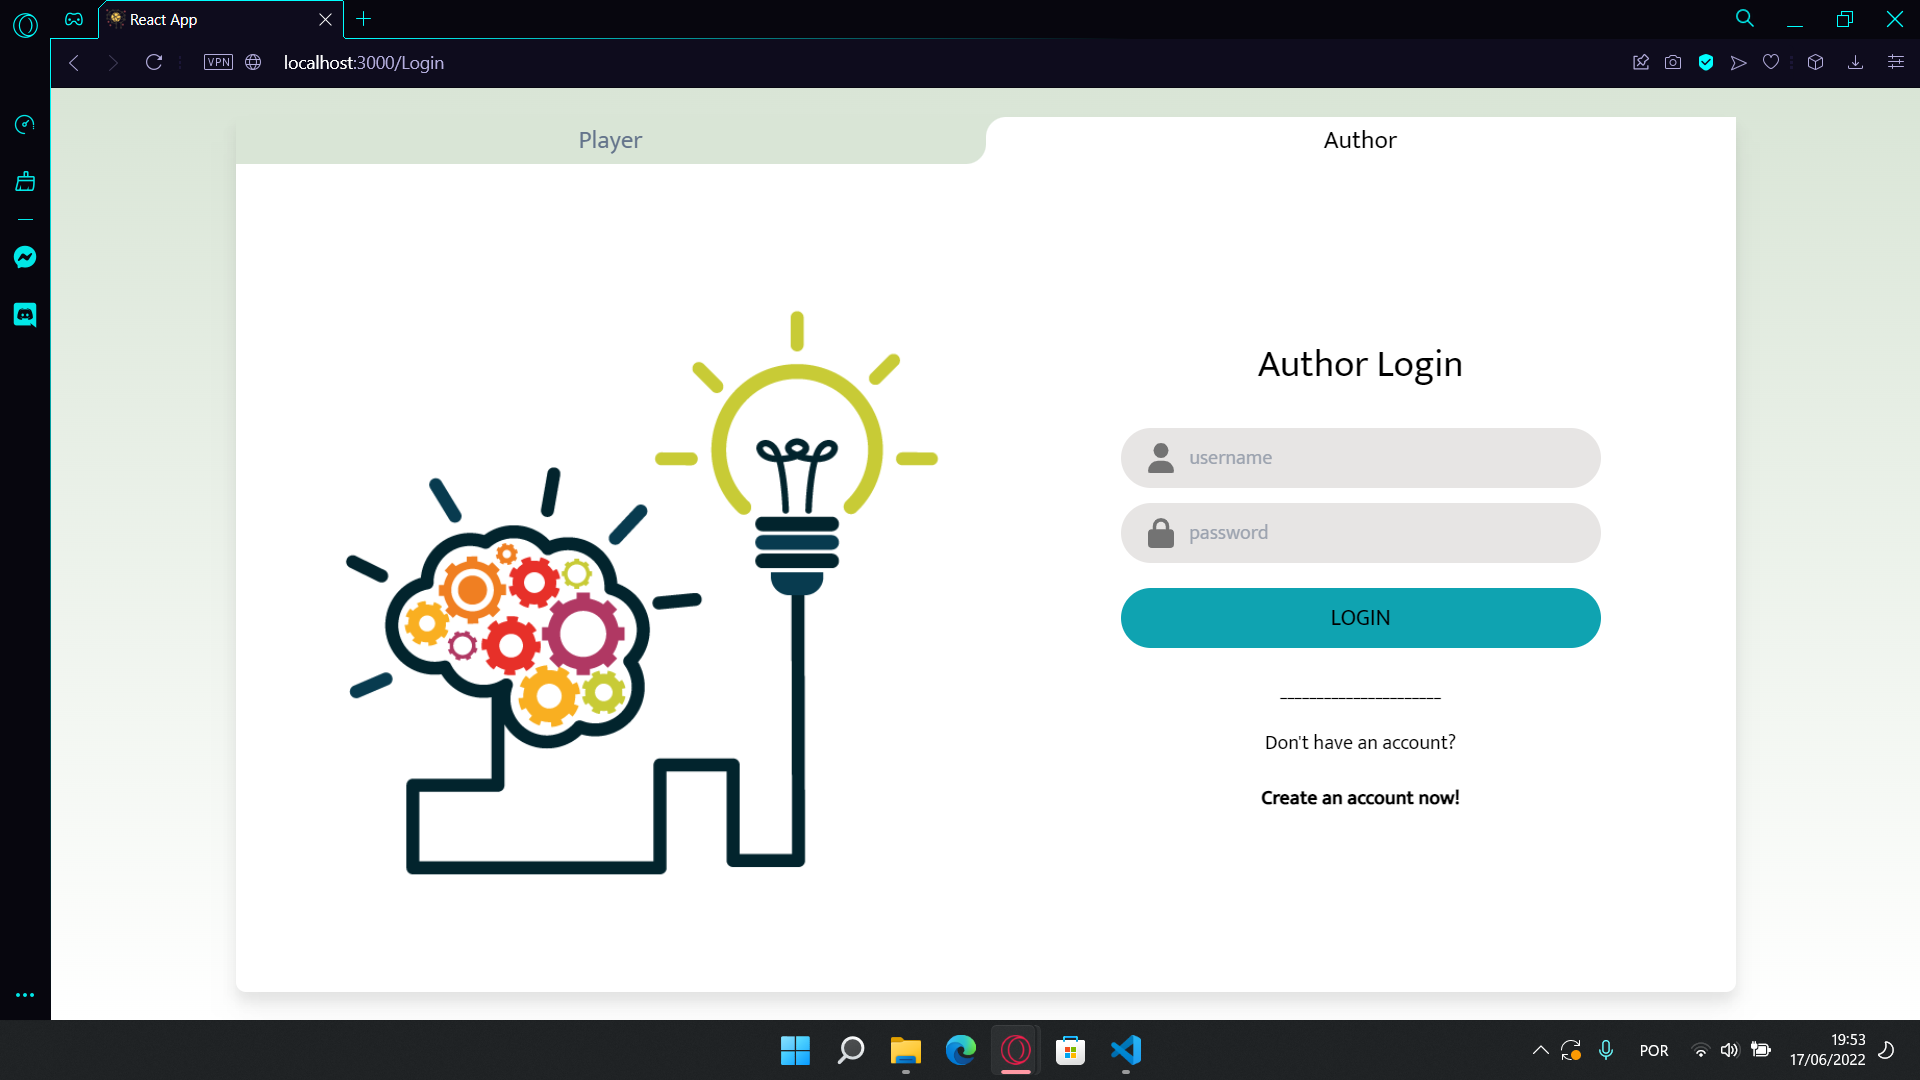
\includegraphics[width=5cm]{log.png} }}%
    \qquad
    \subfloat[\centering Página de \emph{Sign Up Author}]{{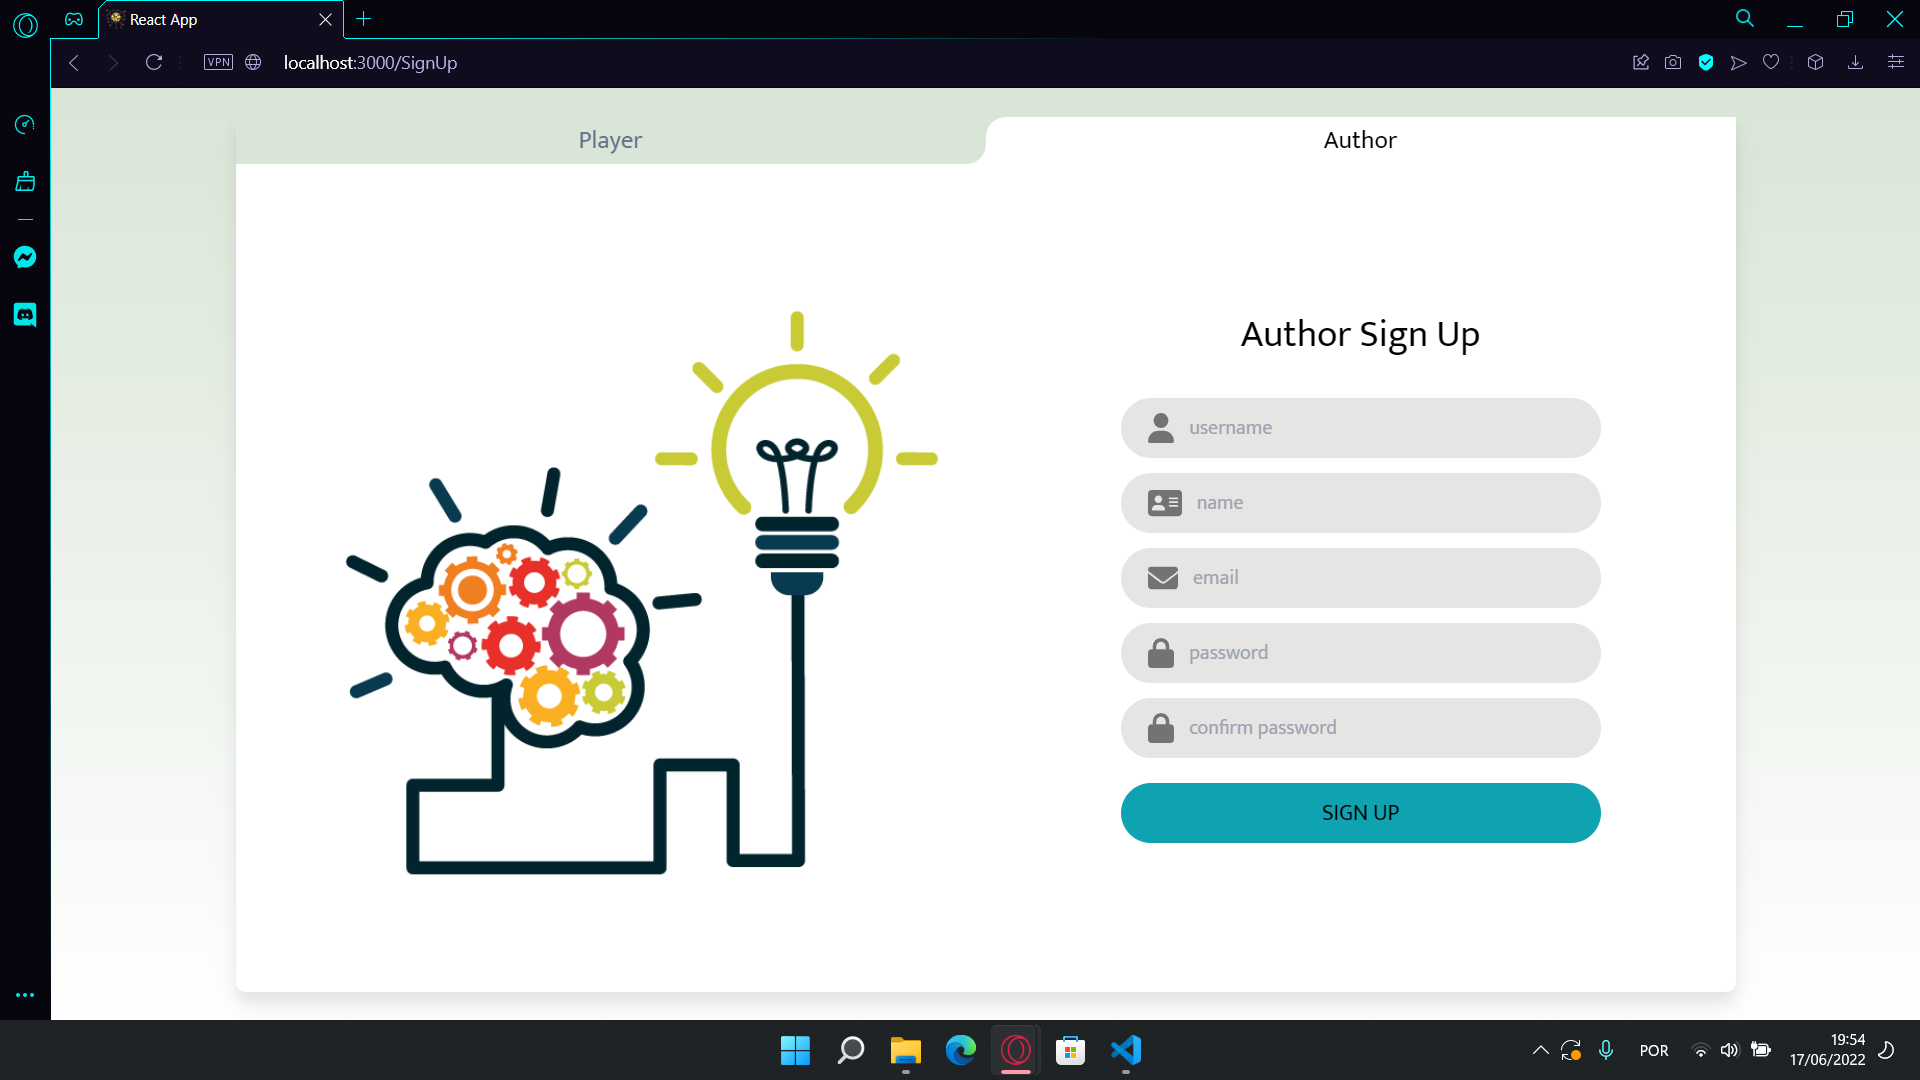
\includegraphics[width=5cm]{sigUpA.png} }}%
    \qquad
    \subfloat[\centering Página de \emph{Sign Up Player}]{{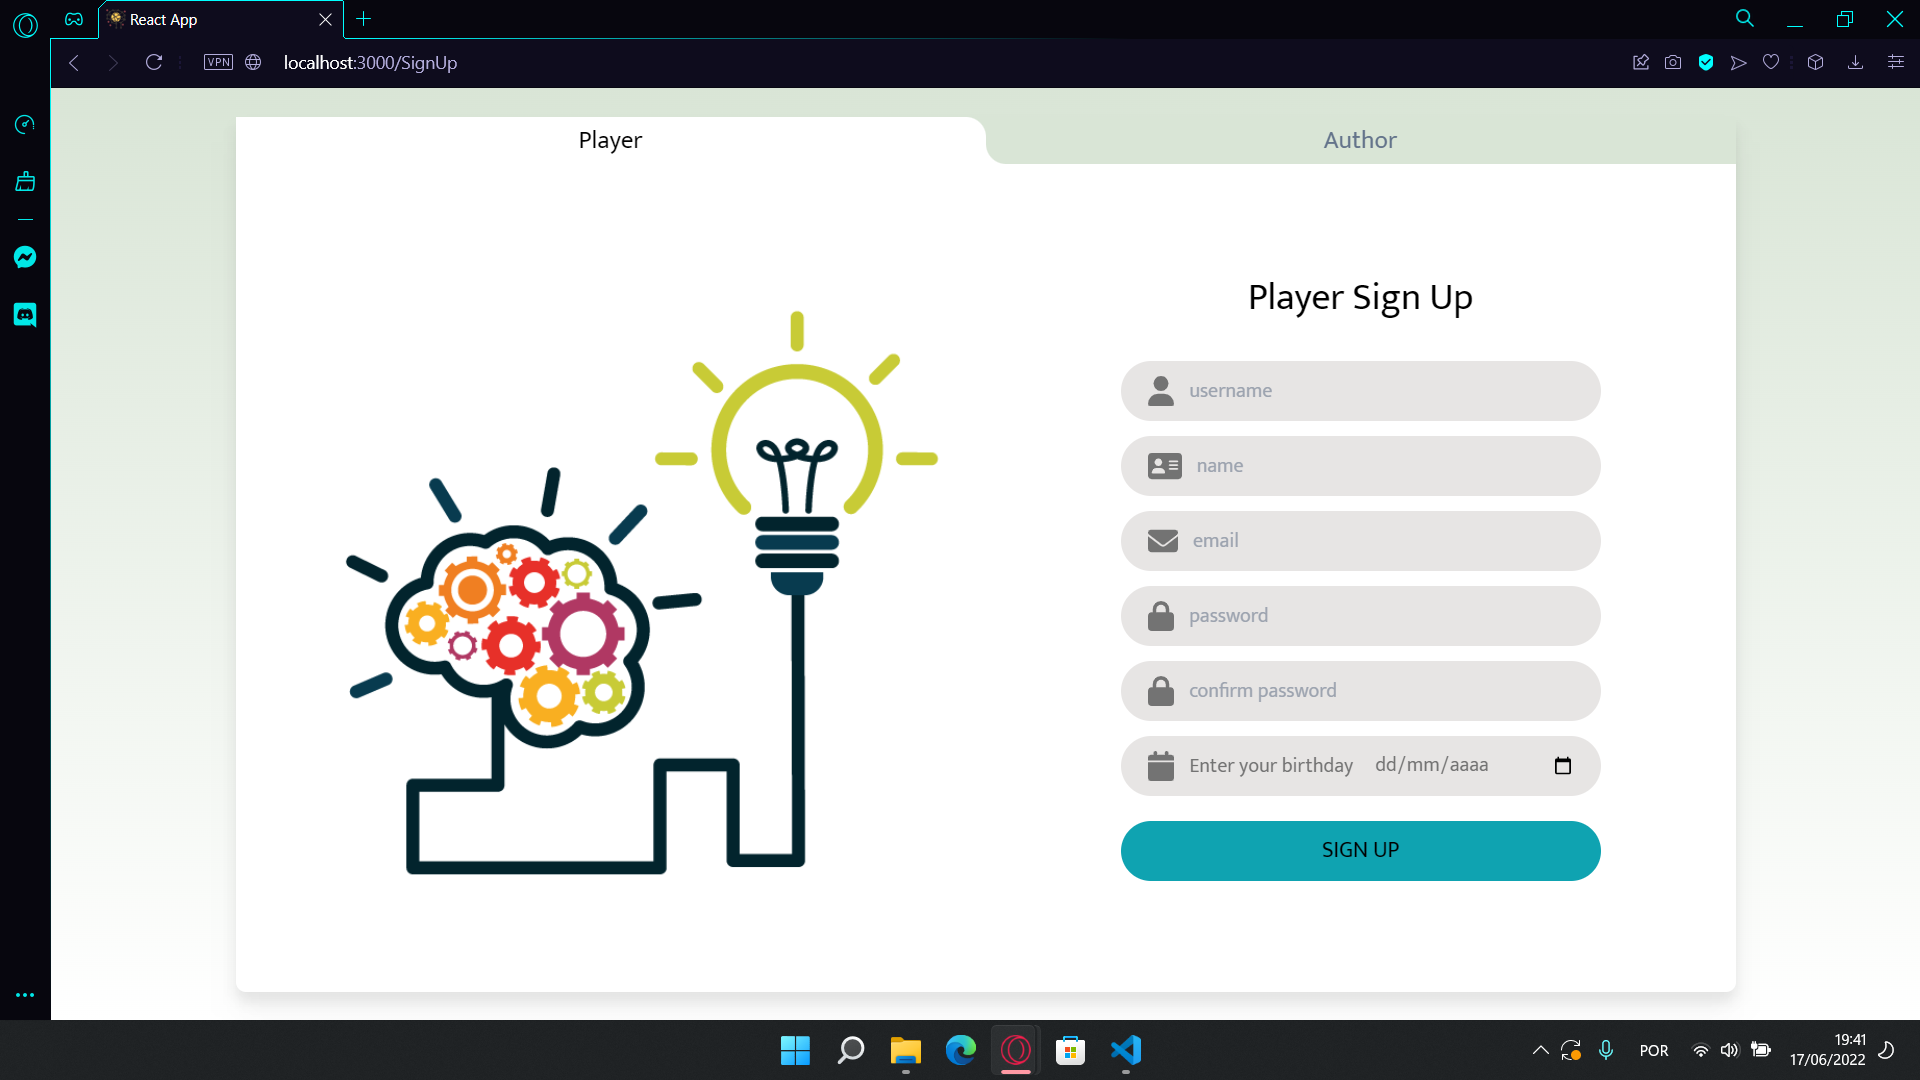
\includegraphics[width=5cm]{sigUpP.png} }}%
    \caption{Página de \emph{Login} e Registo}%
    \label{fig:log&sigUp}%
\end{figure}

\section{Menu do \emph{Author}}
O \emph{Author} é um utilizador especial, diferindo de um utilizador normal pelo facto de existir uma secção chamada \emph{Creat New Game} onde poderá criar os diferentes tipos de jogos referidos nos capítulos anteriores.\newline\newline

\begin{figure}[h]
    \centering
    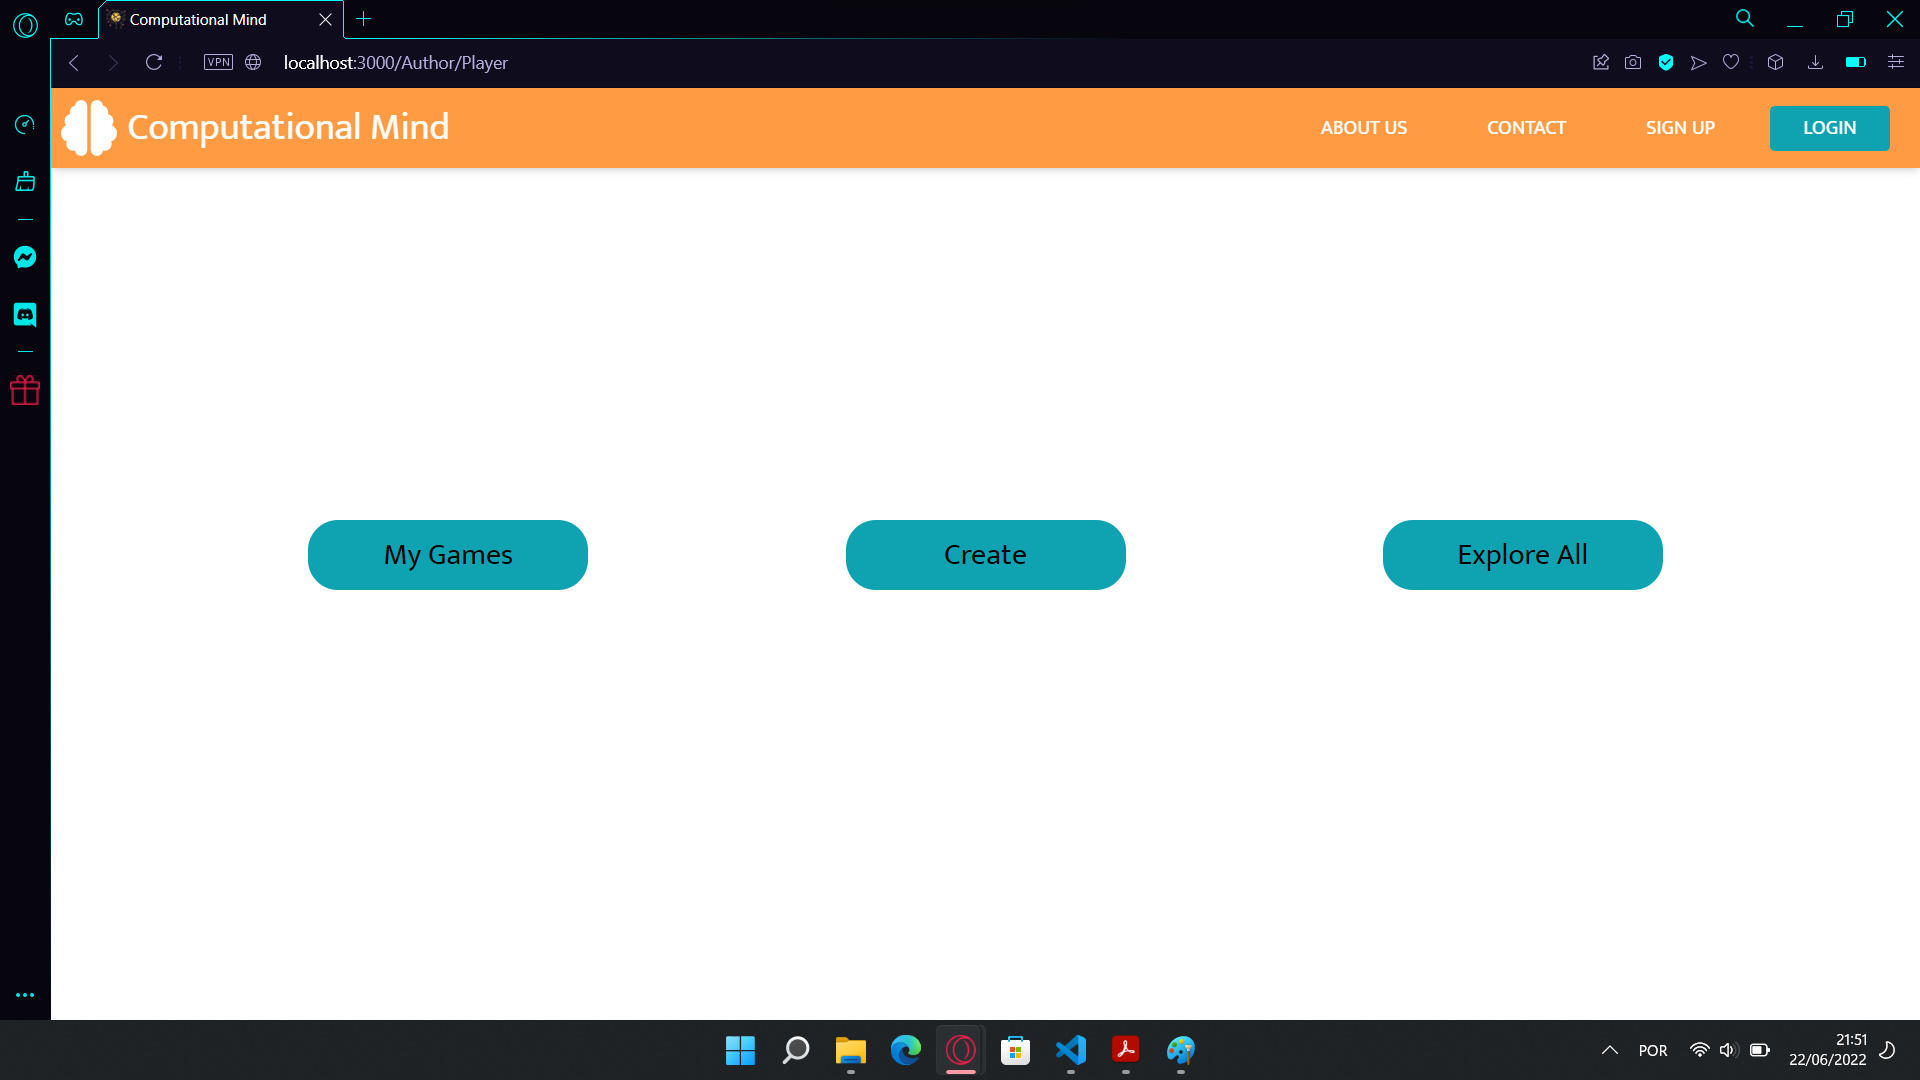
\includegraphics[width = 10cm]{menuAut.png}
    \caption{Menu do \emph{Author}}
    \label{fig:menuAut}
\end{figure}

\newpage

\section{\emph{New Game Menu}}
Neste menu oferecemos todas as ferramentas suportadas pela página para que o \emph{Author} consiga criar novo conteúdo para a mesma.\newline\newline

\begin{figure}[h]
    \centering
    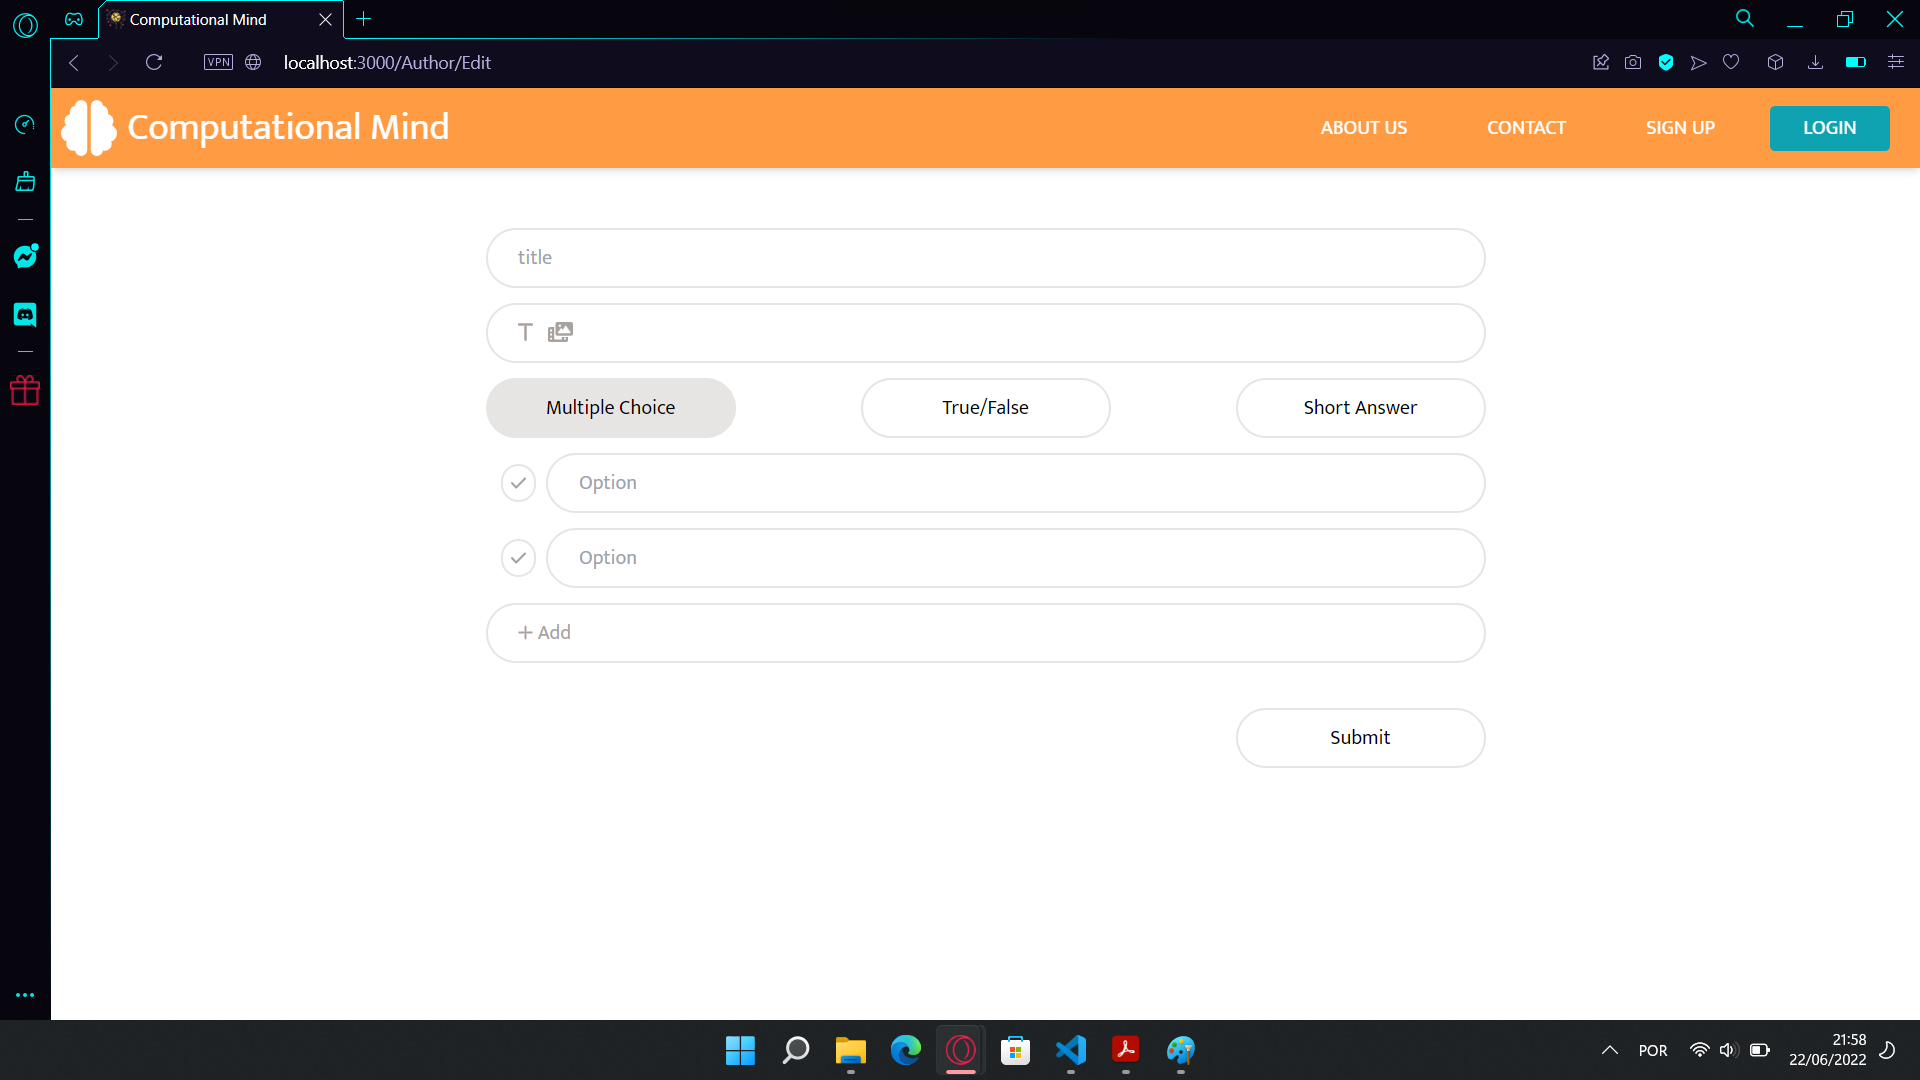
\includegraphics[width = 10cm]{editAut.png}
    \caption{Menu para Criação de Jogos pelo \emph{Author}}
    \label{fig:editAut}
\end{figure}

\section{Menu de jogos para \emph{Player}}
Em seguida, ambos os utilizadores são redirecionados para uma página onde se lista todos os jogos que estão disponíveis para jogar.\newline\newline

\begin{figure}[h]
    \centering
    \includegraphics[width = 10cm]{pagJog.png}
    \caption{Página de Jogos}
    \label{fig:pagJog}
\end{figure}

\section{Página de Jogo}
Nesta página, o \emph{Player} pode fazer a seleção ou a escrita da resposta que pensa ser correta mediante a pergunta enunciada acima.

\begin{figure}[h]
    \centering
    \includegraphics[width = 10cm]{jogJogo.png}
    \caption{Página do Jogo}
    \label{fig:jogJogo}
\end{figure}

\section{Página de \emph{Score}}
Após submeter a sua resposta, o \emph{Player} é presenteado com a sua prestação no jogo. 

\begin{figure}[h]
    \centering
    \includegraphics[width = 10cm]{scoreJogo.png}
    \caption{Página de \emph{Score}}
    \label{fig:scoreJogo}
\end{figure}

\chapter{Conclusão}

Durante a realização deste trabalho constatamos que a parte fundamental para a implementação de um \emph{web site}, de forma coerente, robusta e segura, assenta em algo mais do que um simples \emph{design} atrativo e um \emph{display} de conteúdos, existindo todo um fluxo e uma rede de comunicação que se dá por trás de cada clique ou de cada palavra digitada e enviada, resultando numa relação causa-efeito.

Relativamente às dificuldades sentidas, o principal desafio foi a utilização de uma linguagem de programação e de ferramentas de desenvolvimento de software completamente novas. Consequentemente, foi necessário um grande investimento da nossa parte com o intuito de nos familiarizarmos com estas e de obtermos um resultado final notável.   

Embora tenhamos prestado a devida atenção aos diferentes detalhes, existem, ainda, possíveis melhorias a implementar. Em particular, como o projeto não se encontra totalmente finalizado, consideramos que seria útil a implementação de todas as funcionalidades, que estavam, inicialmente, planeadas e que não estão no produto final. Do mesmo modo, seria igualmente interessante o desenvolvimento de funcionalidades extra que tornassem a página \emph{web} mais apelativa para o utilizador como, por exemplo, a existência de um \emph{ranking} de pontuações adquiridas pelos jogadores nos diferentes quizes, etc.

Em suma, apesar de termos encontrado alguns obstáculos, ao longo deste processo, e de o resultado final ser apenas uma “amostra” daquele que foi inicialmente idealizado, dado que introduzimos apenas as funcionalidades mais importantes,  julgamos ter concluído o projeto com relativo sucesso, na medida em que este se tratava de um projeto ambicioso.

\appendix
\chapter{Exemplos}

\begin{figure}[h]
    \centering
    \includegraphics[width = 15cm]{jog1.png}
    \label{fig:jog1}
\end{figure}

\begin{figure}[h]
    \centering
    \includegraphics[width = 10cm]{jog2.png}
    \label{fig:jog2}
\end{figure}

\begin{figure}[h]
    \centering
    \includegraphics[width = 10cm]{jog3.png}
    \label{fig:jog3}
\end{figure}

\end{document}
